\chapter{Results and Discussion}\label{ch:results_discussion}
This chapter presents the results of our experiments as performed according to the plan described in Chapter~\ref{ch:methods}. Section~\ref{results} provides the data and we then discuss these results in Section~\ref{discussion}. 

\section{Results}\label{results}
In this section we present the results of our experiments. We begin by presenting the results of our statistical analysis before moving on to show the results in various plots. It is of minor note that in many of the figures, a rolling window was used to smooth the values, resulting in many of the plots only showing data starting after a few thousand generations (often 10,000). It should be noted, however, that organisms were continuously evolved for 500,000 generations. 

\subsection{Genome Size}\label{sec:genome_size}
In this section we will examine the results of the different conditions, focusing on which, if any, lead to a reduced genome. Figure~\ref{fig:genome_size} presents the main findings regarding genome size. In the figure, the blue line shows the control condition and the other colors show the changed conditions: $\mu_+$/$\mu_-$ (mutation up/down), $k_+$/$k_-$ (selection up/down), and $N_+$/$N_-$ (population up/down). As can be seen from the figure, our expectations in Section~\ref{sec:expected_results} did not hold up, as all conditions actually \textit{increased} over their original size.
\begin{figure}[H]
	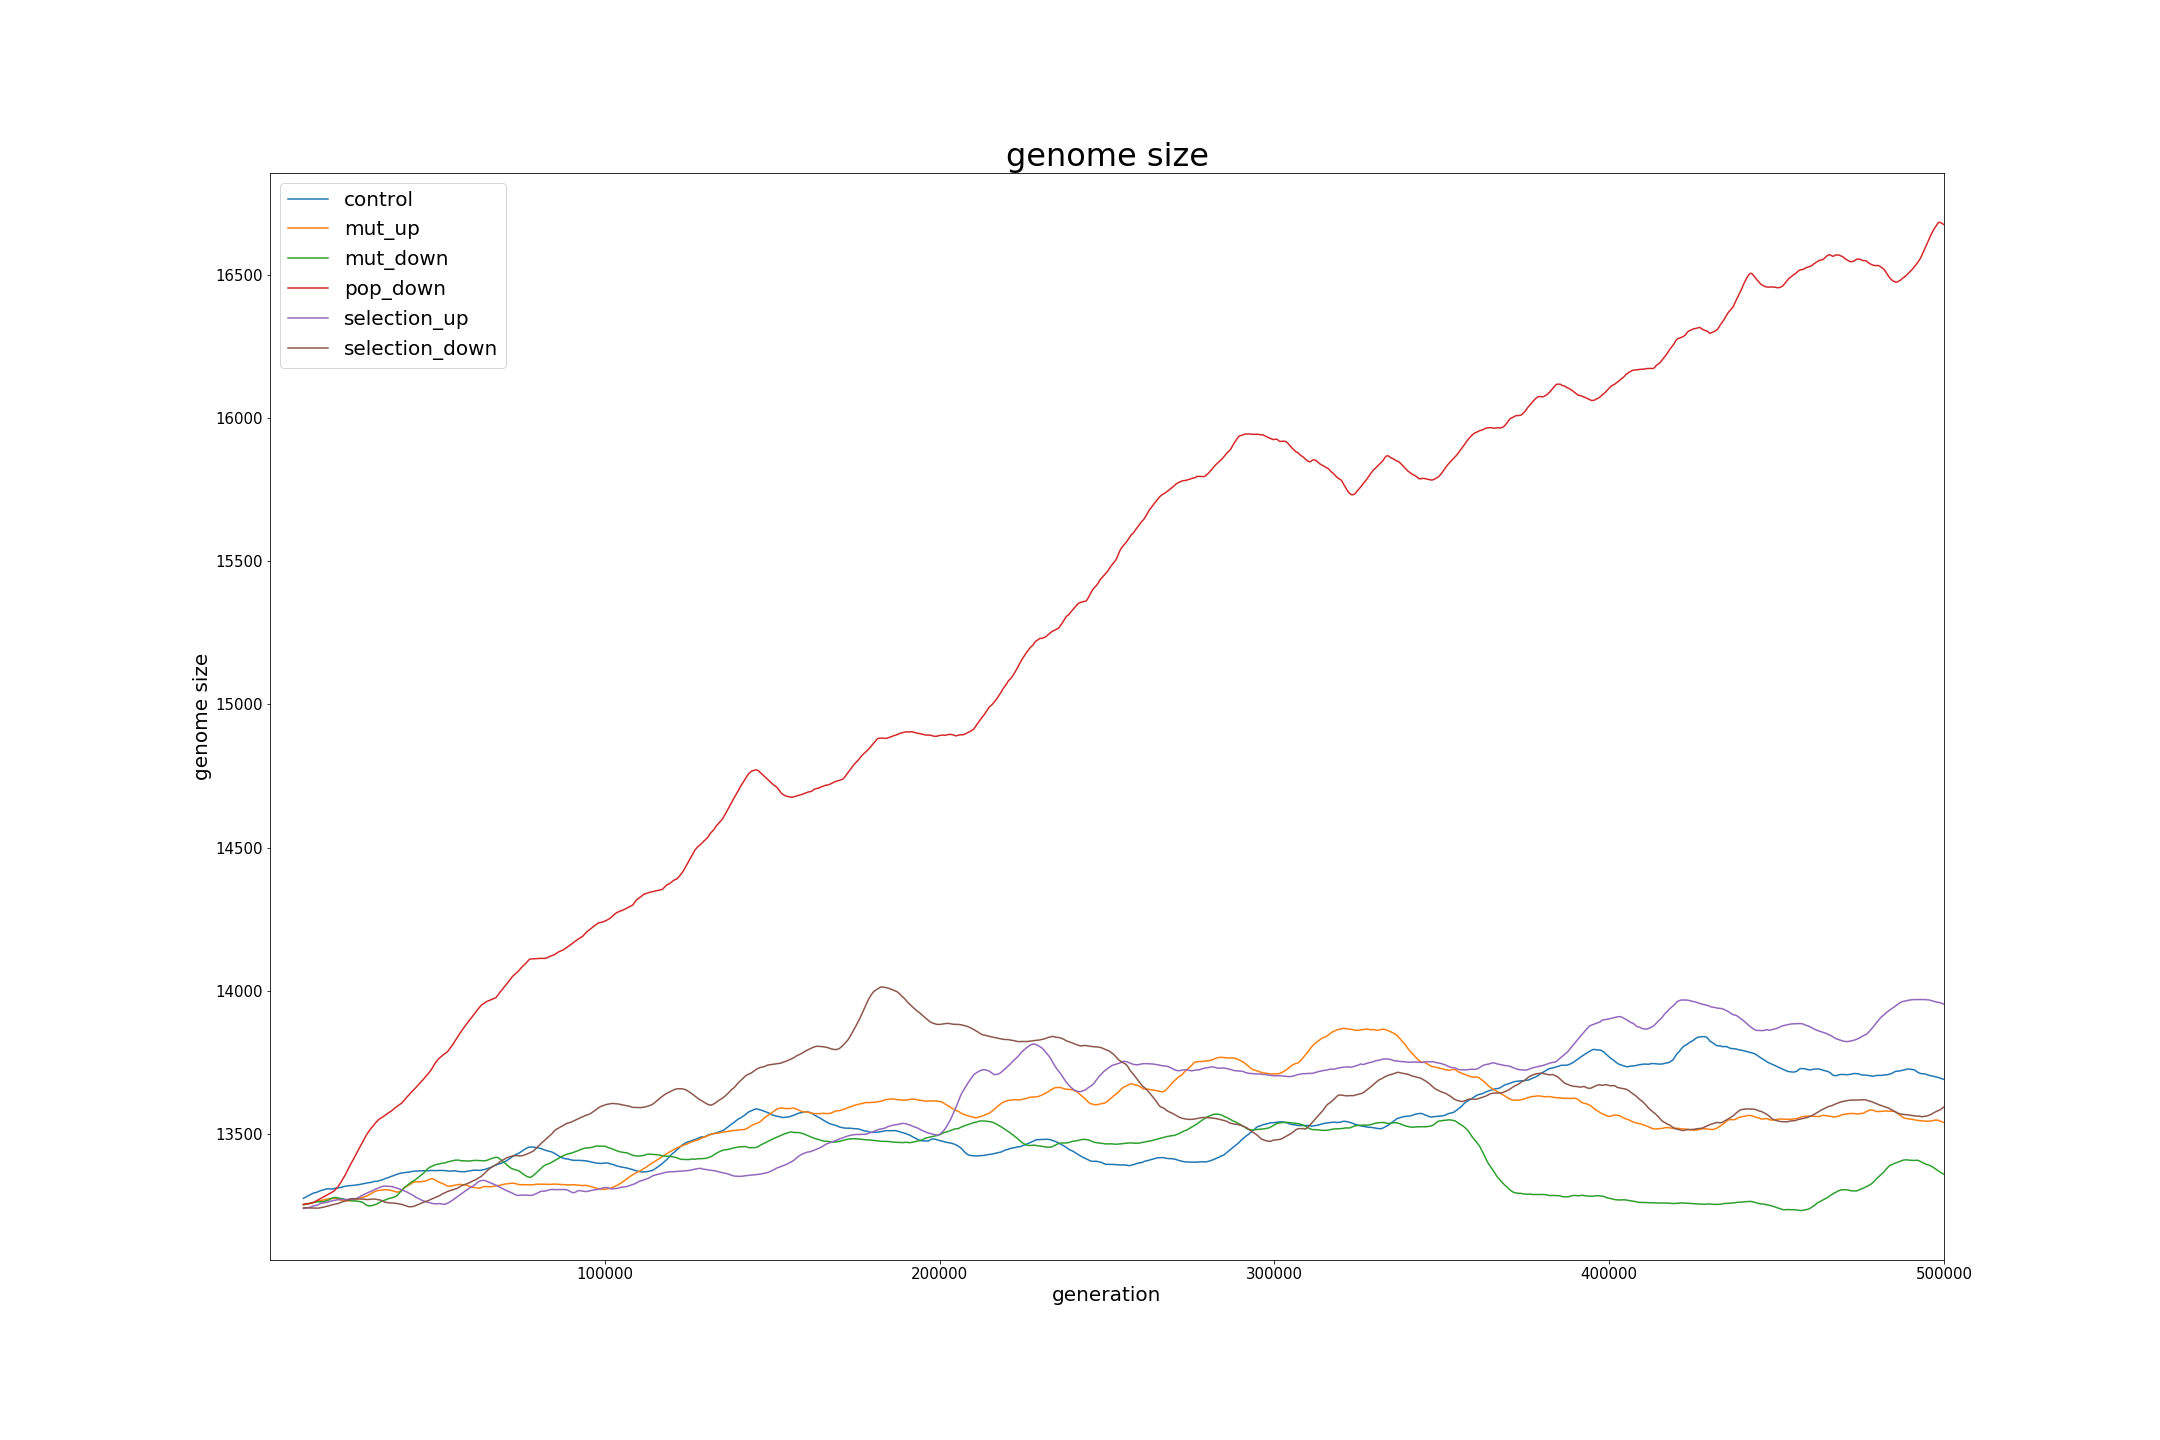
\includegraphics[width=\linewidth]{stat_fitness_global_mean_genome_size}
	\centering
	\caption[Genome size]{Genome size in number of bases of all conditions. Average taken across all five seeds for each condition.}
	\label{fig:genome_size}
\end{figure}
In fact the \textit{population down} condition had a runaway increase in the number of bases, reaching over 16,500 bases at one time, a 25\% increase over the original wild type's roughly 13,200 bp. Surprisingly, even after 500,000 generations it seems that the upper limit may still not have been reached. The statistical results are given below in Tables~\ref{table:genome_size_stats} and \ref{table:genome_size_mean_and_std_dev}, which show the mean and standard deviation among all five seeds.

\begin{table}[H]
	\begin{tabular}{|c|c|c|}
		\hline
		\multicolumn{3}{c}{\Large \textbf{Genome Size - Mean \& Std. Dev. (in bp)}} \\
		\hline
		 & \textbf{mean} & \textbf{standard deviation} \\
		 \hline
		 Control & 13537.031513461712 & 144.35113788568995 \\
		 \hline
		 $\mu_+$ & 13558.37415989583 & 155.0778470373894 \\
		 \hline
		 $\mu_-$ & 13410.74368980468 & 101.37610437279282 \\
		 \hline
		 $k_+$ & 13621.901103597776	& 229.63570760641895 \\
		 \hline
		 $k_-$ & 13614.663598682531 & 172.67504183409068 \\
		 \hline
		 $N_-$ & 15275.14939195188 & 950.2662434333312 \\
		 \hline
	\end{tabular}
	\caption[Genome size - mean and std. dev.]{Average genome size and standard deviation for all seeds and all conditions. }
	\label{table:genome_size_mean_and_std_dev}
\end{table}

\begin{table}[H]
	\centering
	\begin{tabular}{|c|c|c|}
		\hline
		\multicolumn{3}{c}{\Large Genome Size - Rank Sum \& P-Values} \\
		\hline
		& \textbf{rank sum U} & \textbf{p-value} \\
		\hline \hline
		$\mu_+$ & 110508011469.5 & 0.00000000000000 \\
		\hline
		$\mu_-$ & 71008638349.5 & 0.00000000000000 \\
		\hline
		$N_-$ & 16477791900.5 & 0.00000000000000 \\
		\hline
		$k_+$ & 100151680984.5 & 0.00000000000000 \\
		\hline
		$k_-$ & 88533681875.0 & 0.00000000000000 \\
		\hline
	\end{tabular}
	\caption[Genome size statistics]{Genome size statistics. Each condition is compared with the \textit{control} condition.}
	\label{table:genome_size_stats}
\end{table} 

The next most obvious observation is that of the remaining conditions, all but the \textit{selection up} condition (which had an an increase of 11\% over the control condition) ended up with fewer base pairs than the control condition, though all increased slightly over their starting point. Also noteworthy is that the mutation down condition appears to have had a steady increase in the number of base pairs until a maximum of just over 14,000 around generation 350,000 before having a fairly sharp decline back to nearly the original size. 

Examining the percent changed from the \textit{control} condition shown in Figure~\ref{fig:genome_size_percent_change} we see that at points, the \textit{mutation down} condition was nearly 5\% smaller than the \textit{control} condition. 

\begin{figure}[H]
	\centering
	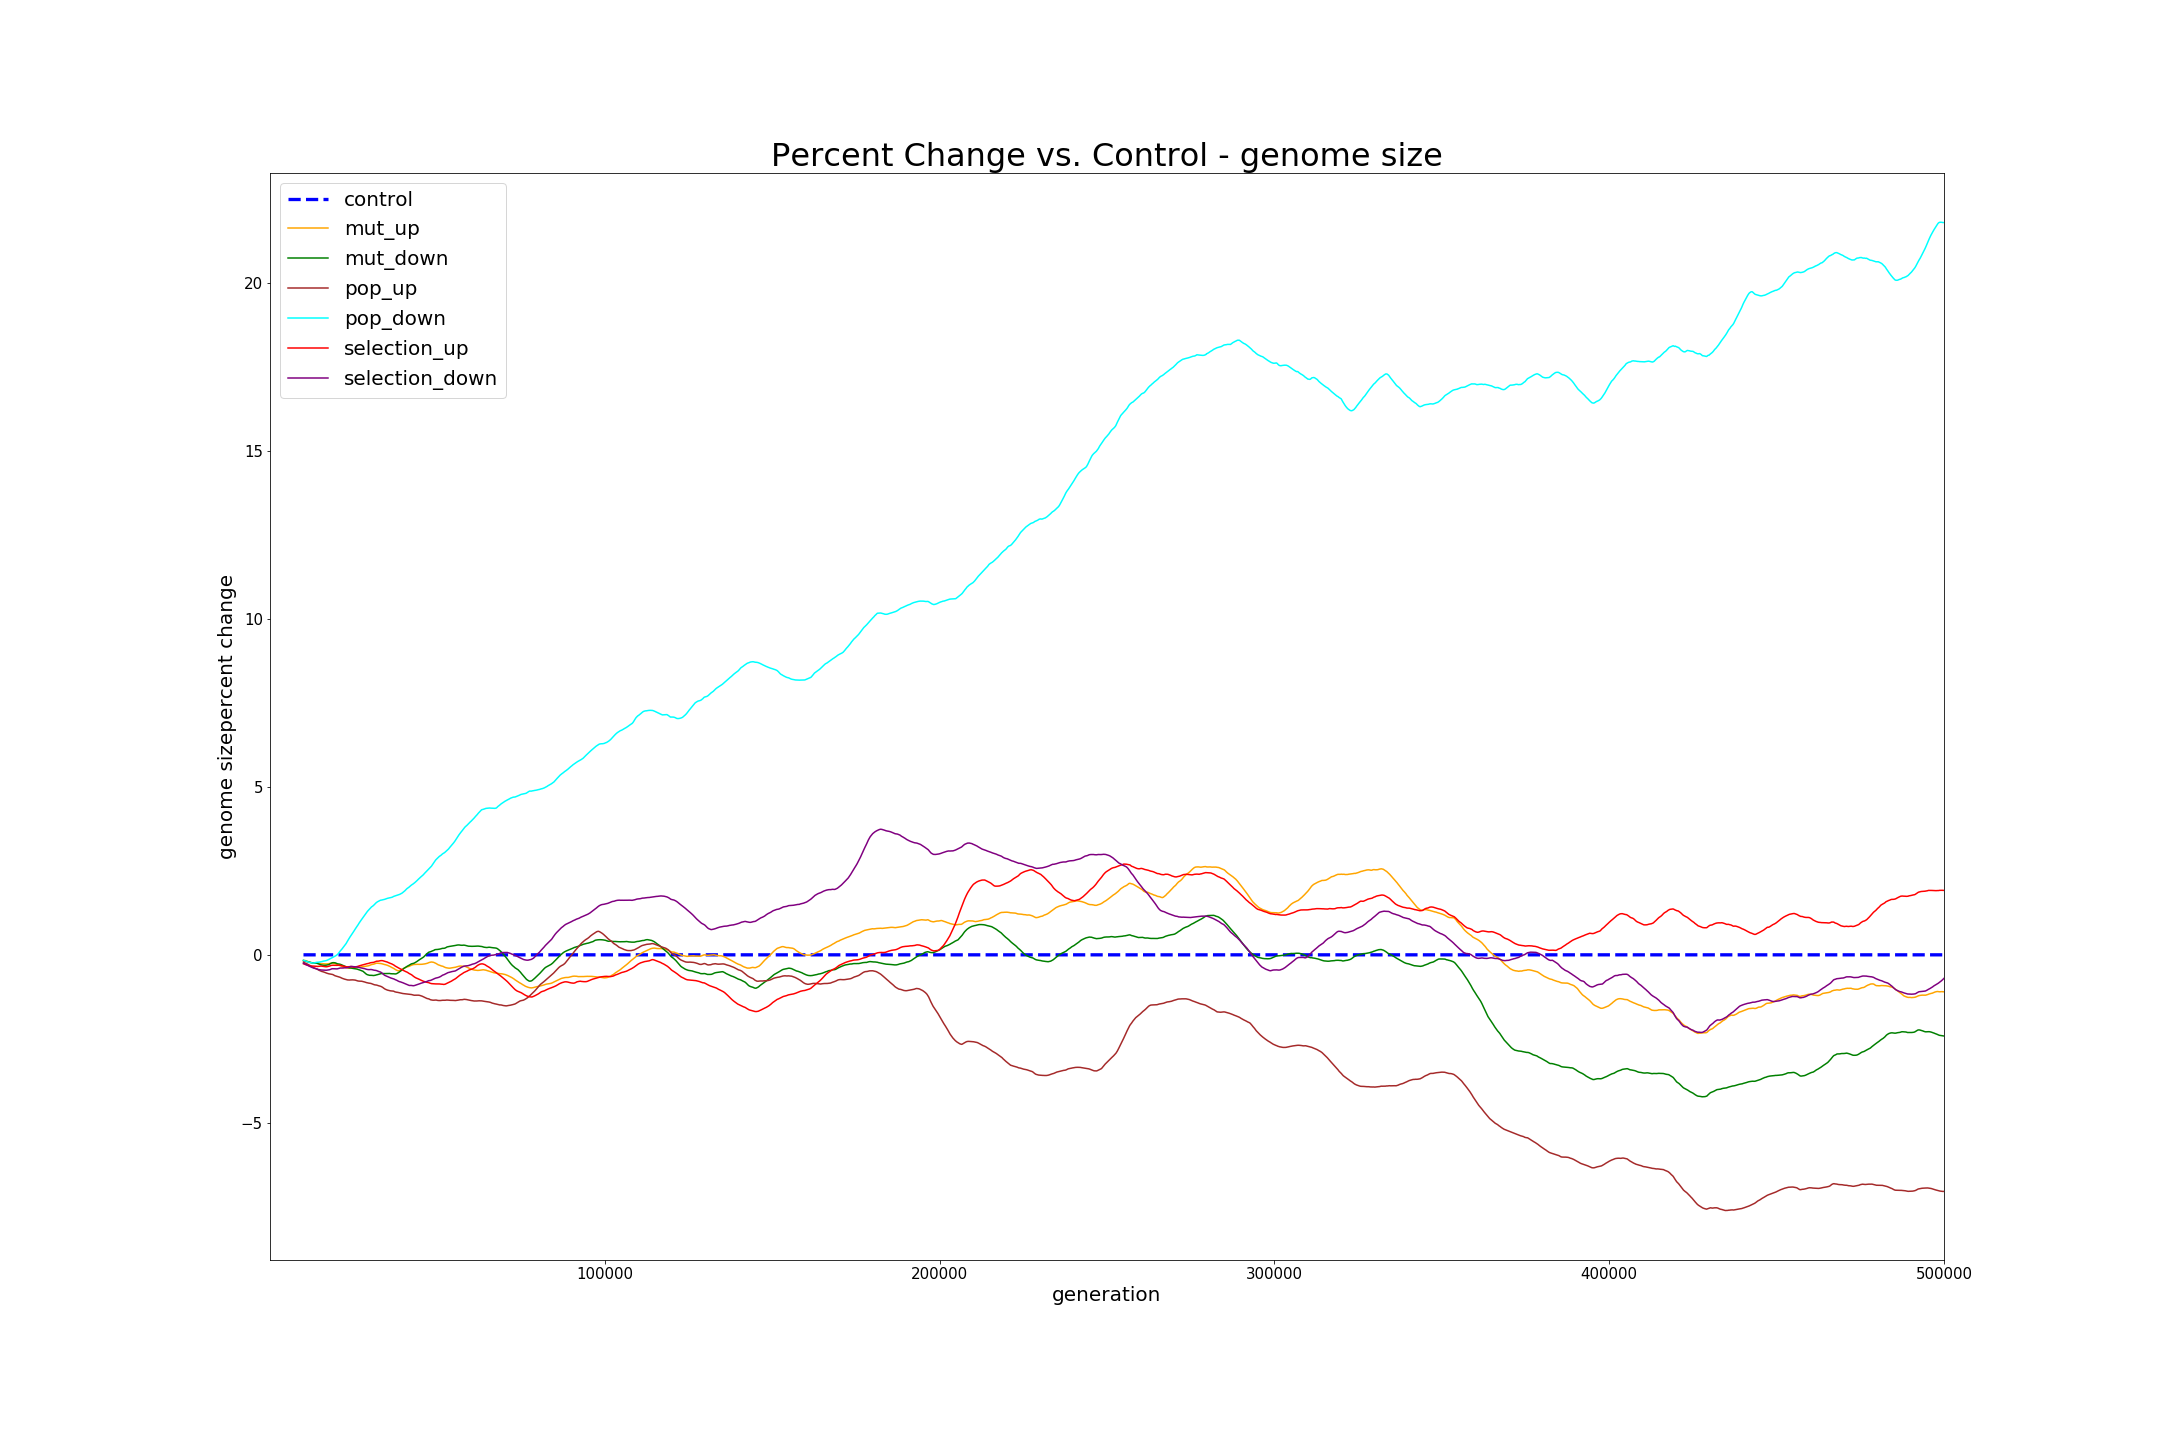
\includegraphics[width=\linewidth]{stat_fitness_perc_change_genome_size}
	\caption[Genome size - percent change]{Genome size's percent change from the \textit{control} condition.}
	\label{fig:genome_size_percent_change}
\end{figure}


\subsection{Metabolic Error and Fitness}
Figure~\ref{fig:mean_fitness_plot} shows the mean fitness of the population for the control, mutation up/down, and population down conditions. Selection up/down were excluded from this graph because they were significantly outside of the range of the other conditions and made the results impossible to graph, but they are included in Figure~\ref{fig:global_fitness_histogram}, a histogram of the results.

\begin{figure}[H]
	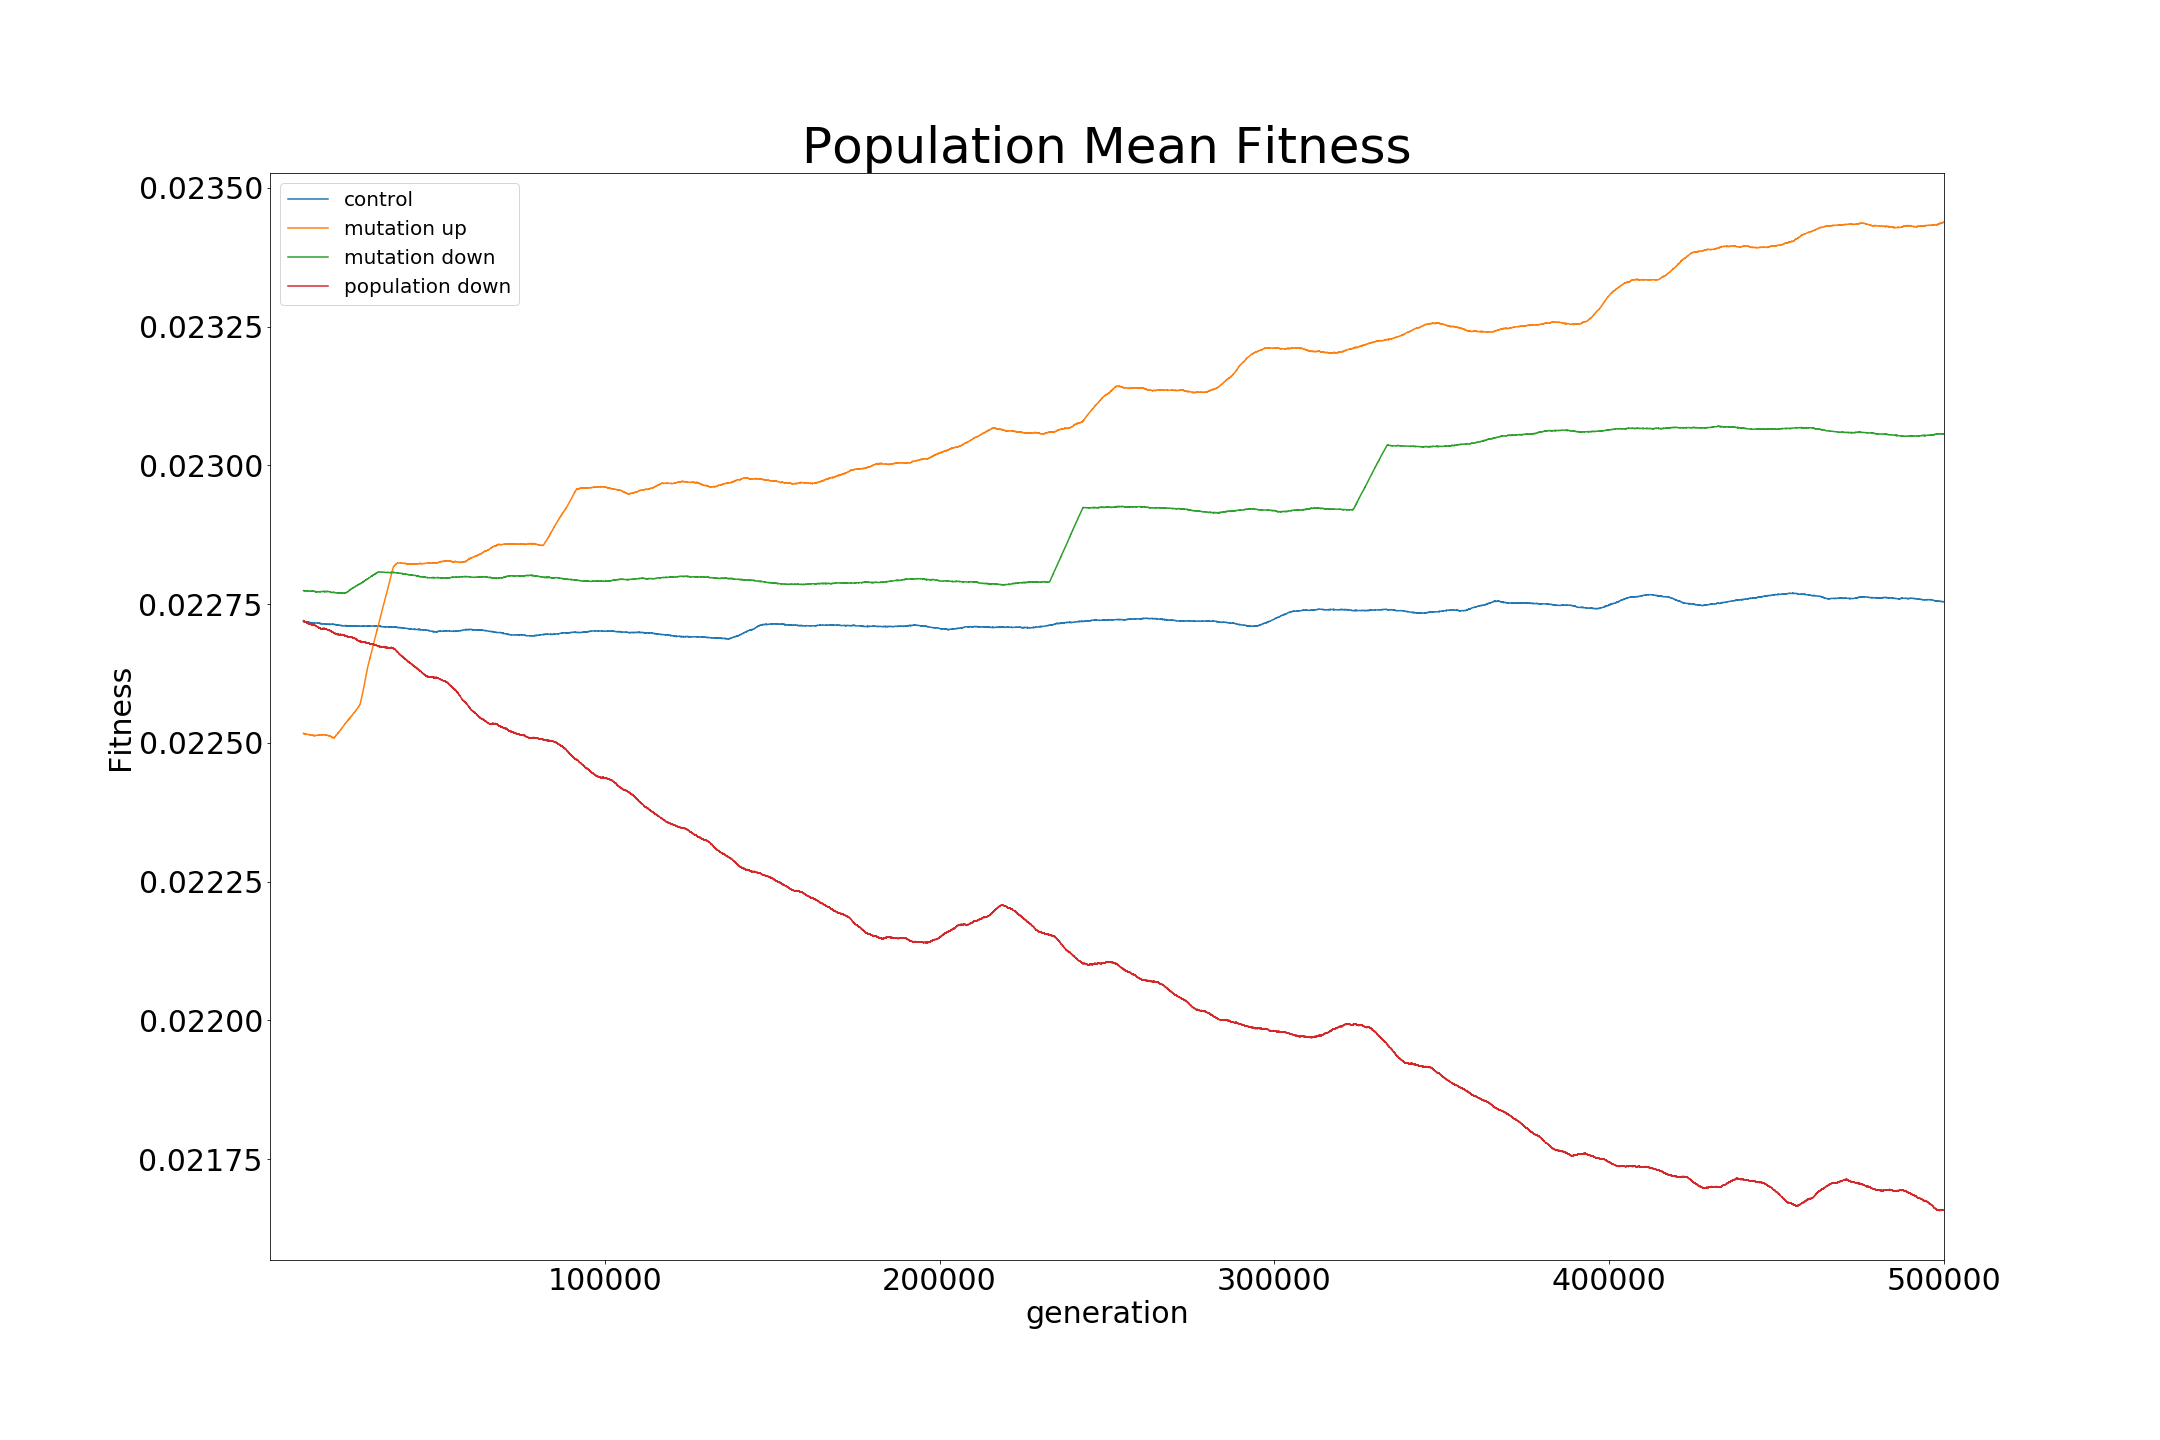
\includegraphics[width=\linewidth]{population_mean_fitness_chart}
	\caption[Mean fitness]{Plot of the mean fitness over time for the control, mutation up/down, and population down conditions.}
	\label{fig:mean_fitness_plot}
\end{figure}

We can see in the figure that the fitness of the control condition (in blue) consistently stayed at the same level, likely owing to the fact that the wild genotype had already been allowed to evolve for 10 million generations in this environment, so the phenotype closely lines up with the target before the simulations even began. Small fluctuations occurred due to mutations, insertions, etc. but since we were beginning with a clonal population of the best organism after 10 million generations in this environment, the average fitness remained steady. 

More interesting is the population down condition, where the average fitness in the whole population sharply declined, sinking to 4.5\% below the control condition at generation 500,000. It seems that with the smaller population size, genetic drift may be more strongly at work in continually increasing the gap between the phenotype and environmental function, as the lack of variety inherent in a smaller population causes a cascade of increasingly deleterious consequences. 

\begin{figure}[H]
	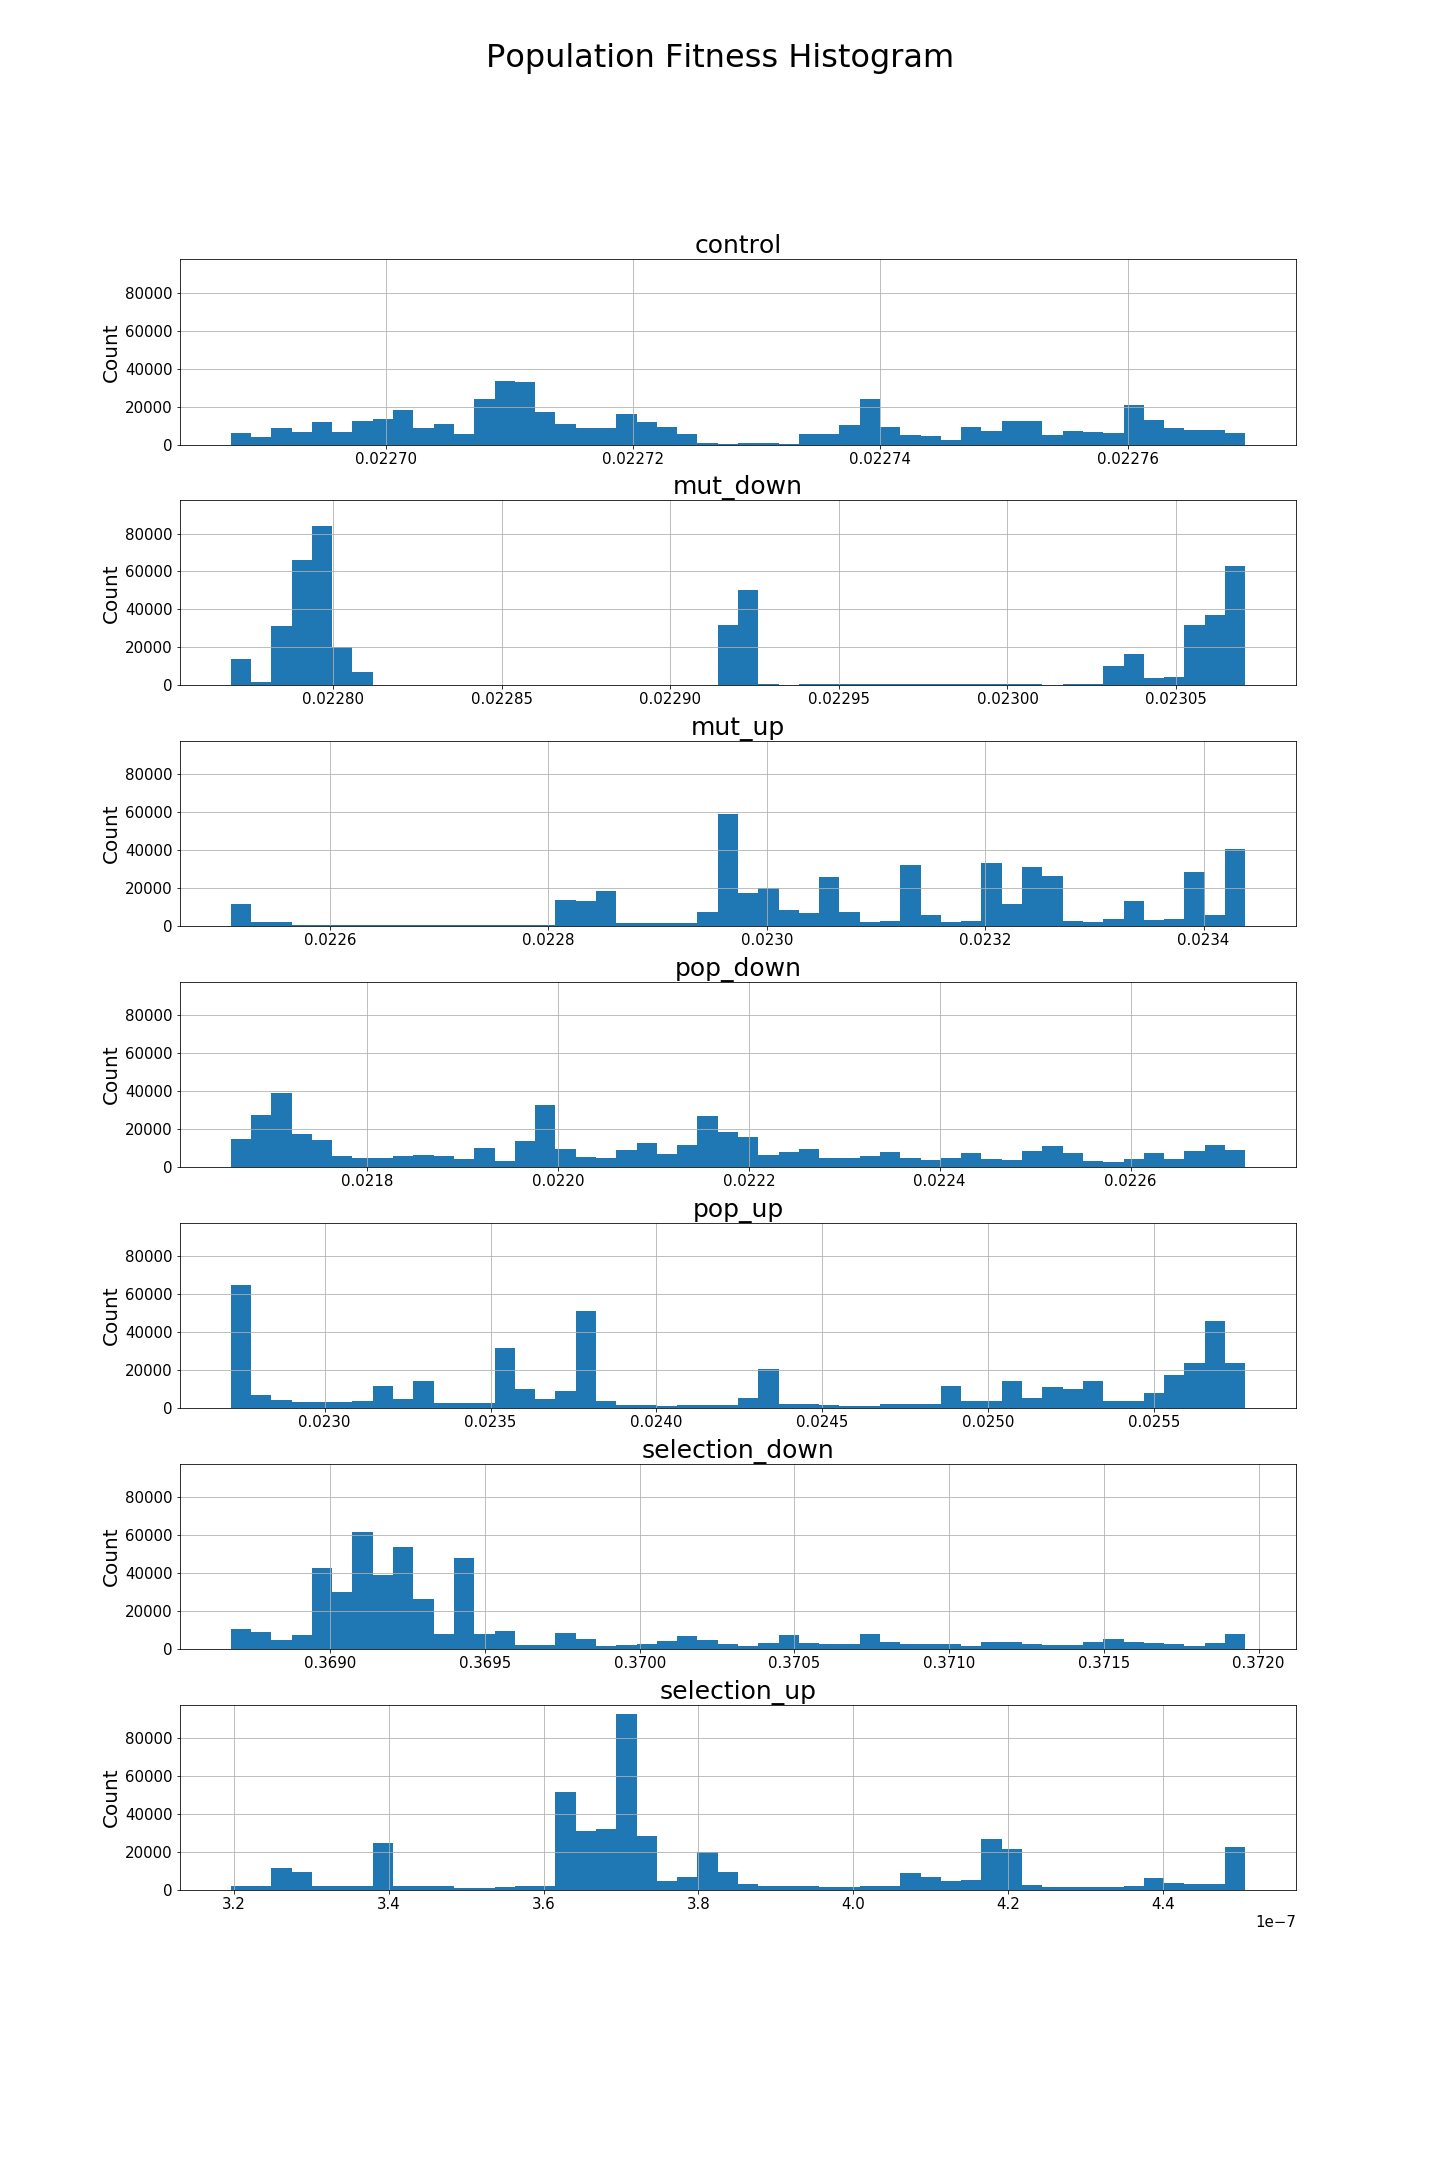
\includegraphics[width=\linewidth]{global_fitness_histogram}
	\caption[Mean fitness histogram]{Histogram of all conditions' fitness. Note that for the selection up condition, the scale is 1e-7. }
	\label{fig:global_fitness_histogram}
\end{figure}
Figure~\ref{fig:global_fitness_histogram} shows a histogram of all fitness values for all conditions. Although the \textit{mutation down} condition ended the simulations in the most similar position to the \textit{control} condition, Figure~\ref{fig:global_fitness_histogram} makes it clear that the \textit{control} condition remained much steadier throughout the simulation, regularly jumping from value to value, whereas the \textit{mutation down} condition, as expected, tended to hover at certain locations in between rarer mutation events. 

Figure~\ref{fig:mean_metabolic_error} shows the mean metabolic error across all seeds for the whole population over time with respect to each condition. 
\begin{figure}[H]
	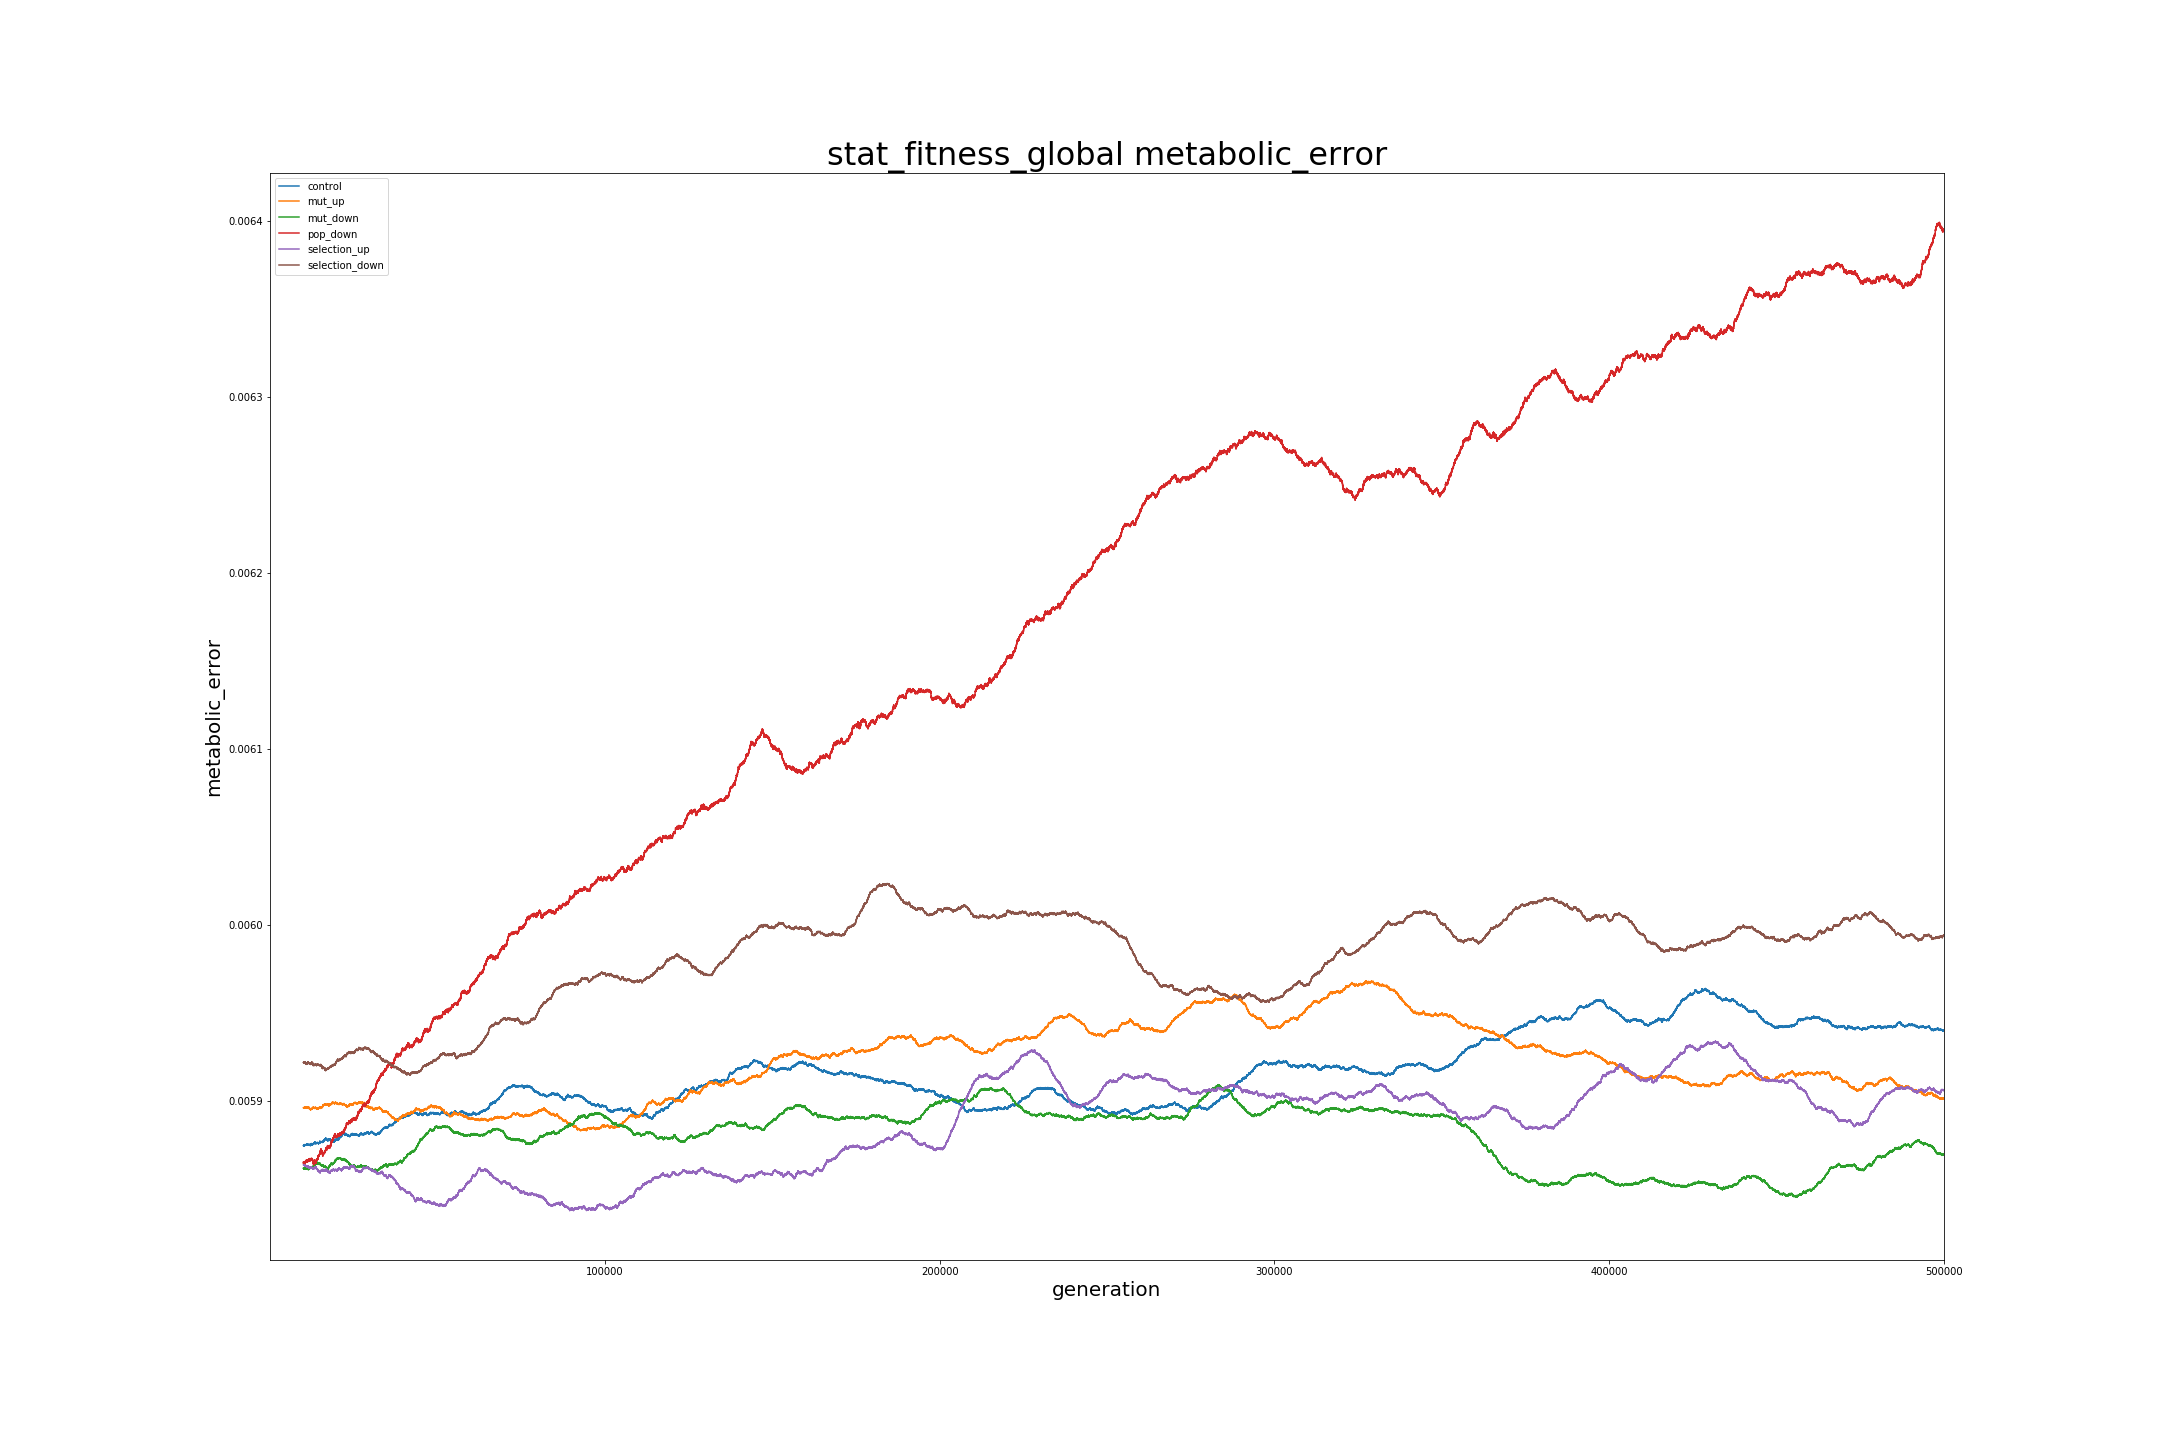
\includegraphics[width=\linewidth]{stat_fitness_global_mean_metabolic_error}
	\caption[Metabolic error]{Plot of the metabolic error over time for all conditions, average of all seeds}
	\label{fig:mean_metabolic_error}
\end{figure}

Table~\ref{table:fitness_means_std_dev} below gives the mean fitness scores for differing conditions. The selection up/down conditions seem to be somewhat anomalous.
\begin{table}[H]
	\centering
	\begin{tabular}{|c||c|c|}
		\hline
		\multicolumn{3}{c}{\Large \textbf{Fitness}} \\
		\hline
		& \textbf{mean} & \textbf{standard deviation} \\
		\hline \hline
		control & 0.022725416617759595 & 2.3443283583311204e-05 \\
		\hline
		$\mu_+$ & 0.02310700617283088 & 0.00021918255246890017 \\
		\hline
		$\mu_-$ & 0.022908786914463554 & 0.0001180940074554785 \\
		\hline
		$k_+$ & 3.803823317637301e-07 & 3.130503751740127e-08 \\
		\hline
		$k_-$ & 0.3695935240107418	& 0.0008101731945386823 \\
		\hline
		$N_-$ & 0.02209722426327717 & 0.00031042637566743275 \\
		\hline
	\end{tabular}
	\caption[Fitness means and standard deviations.]{Fitness means and standard deviations across all seeds. }
	\label{table:fitness_means_std_dev}
\end{table}

\subsection{Genome Structure}
In this section we examine the effects of the differing conditions on the structure of the genome as measured by the criteria in Tables~\ref{table:aevol_stats_genes_and_bp} and~\ref{table:aevol_stats_fitness_and_mutation}. 

\subsubsection{Non-coding DNA}
One important factor in genome structure is the amount of non-coding DNA, i.e. the number of bases which are part of a genome but which do not encode protein sequences. Aevol gives the number of bases which are not in any coding sequence, as well as the total genome size, so one may easily calculate this percentage. The results from our experiments are shown in Figure~\ref{fig:mean_non-coding_DNA}. Recalling genome size in Figure~\ref{fig:genome_size}, it seems that as the genome size of the population down condition rapidly expanded, most of those expansions were non-coding.
\begin{figure}[H]
	\centering
	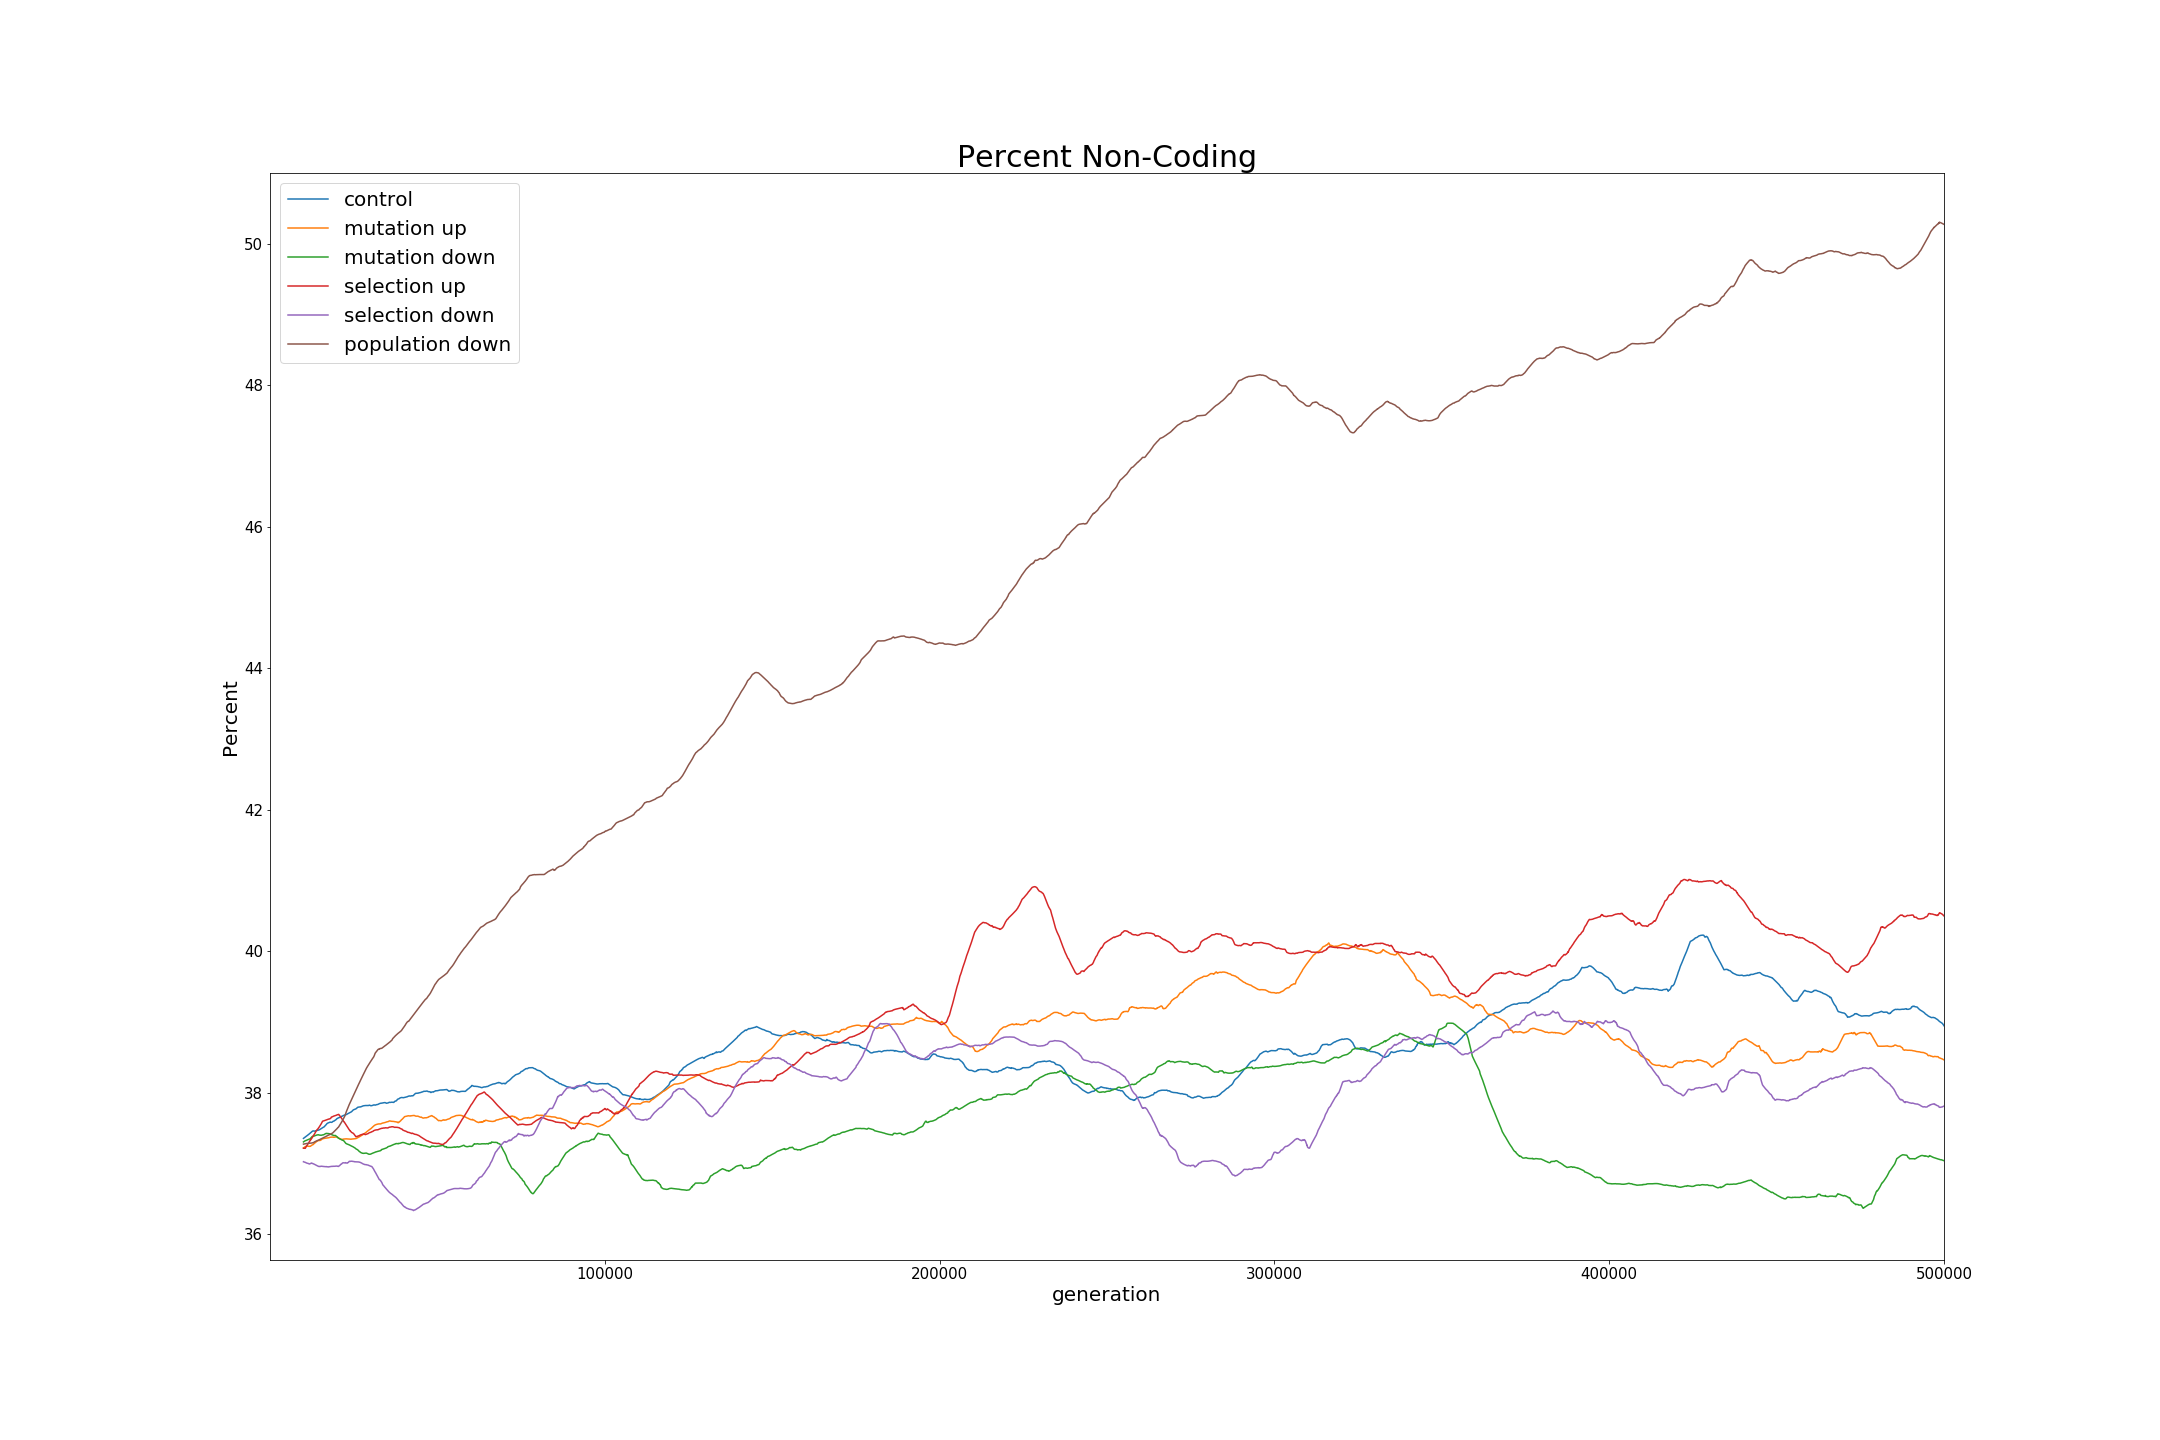
\includegraphics[width=\linewidth]{percent_noncoding}
	\caption[Non-coding DNA]{Plot of non-coding DNA over time for all conditions, average of all seeds.}
	\label{fig:mean_non-coding_DNA}
\end{figure}
By comparison, despite the \textit{selection up} condition's rapid decline in fitness, it did not acquire more than 1\% non-coding DNA. 

The average percentages of non-coding DNA are given in Table~\ref{table:non-coding_DNA_mean_and_standard_deviation} below. 
\begin{table}[H]
	\begin{tabular}{|c|c|c|}
		\hline
		\multicolumn{3}{c}{\Large \textbf{\% Non-coding DNA}} \\
		\hline
		& \textbf{mean} & \textbf{standard deviation} \\
		\hline \hline
		Control & 38.63423466698755	& 0.6082140361213884 \\
		\hline
		$\mu_+$ & 38.671613712955356 & 0.7101004314162586 \\
		\hline
		$\mu_-$ & 37.45404807887061 & 0.6975468467601527 \\
		\hline
		$k_+$ & 39.33999462052945 & 1.135781531861679 \\
		\hline
		$k_-$ & 38.01289386160514 & 0.704172791027157 \\
		\hline
		$N_-$ & 45.46747213756932 & 3.5462787275316896 \\
		\hline
	\end{tabular}
	\caption[Non-coding DNA mean and standard deviation]{Mean and standard deviation of non-coding percentages of DNA across all seeds.}
	\label{table:non-coding_DNA_mean_and_standard_deviation}
\end{table}

\subsubsection{Number of Functional Genes}\label{sec:number_of_functional_genes}
Figure~\ref{fig:mean_num_functional_genes} below illustrates the mean number of functional genes across the population for each condition.  
\begin{figure}[H]
	\centering
	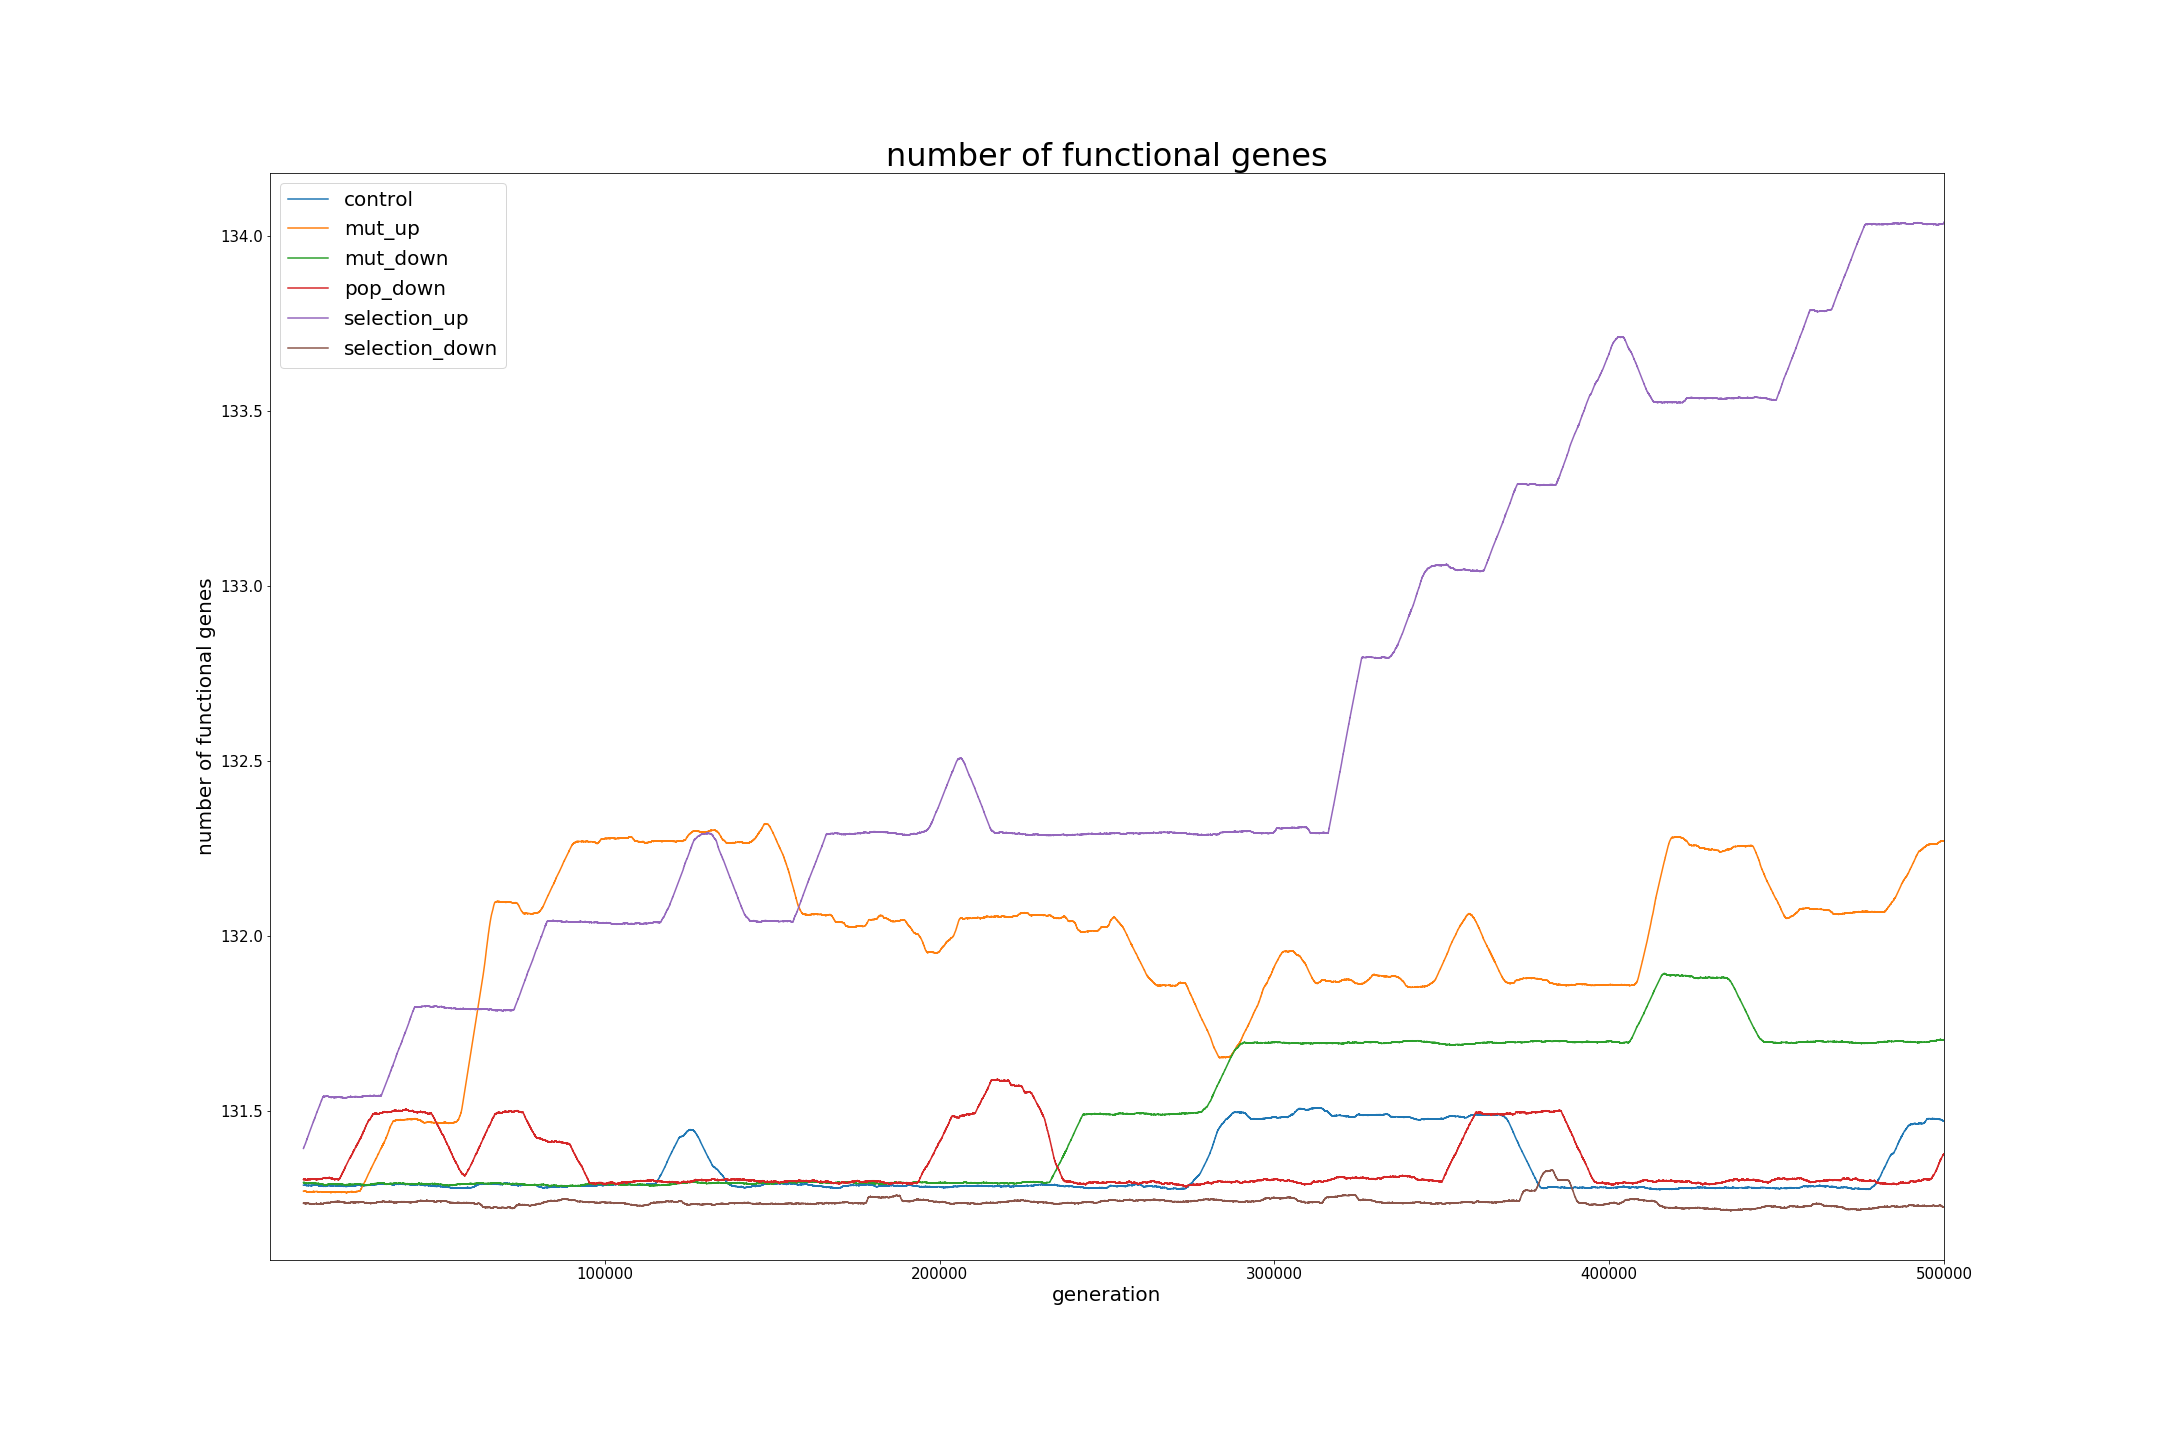
\includegraphics[width=\linewidth]{stat_genes_global_mean_num_functional_genes}
	\caption[Mean number of functional genes]{Plot showing the mean number of functional genes over time across all seeds.}
	\label{fig:mean_num_functional_genes}
\end{figure}
As seen in the figure, the \textit{selection up} condition showed the greatest increase in the number of functional genes in the whole population, reaching a maximum increase of about 2.2\% (131 to 134). This is in agreement with our predictions (from Table~\ref{table:experiment_predictions}) and the findings of Knibbe et al.~\cite{Knibbe2007}. Whereas most of the other curves are fairly flat, the mutation up condition fluctuates relatively rapidly, owing to the quick increase and decrease in the number of base pairs. 

The mean and standard deviation of each condition is given in Table~\ref{table:number_of_genes_mean_std_dev} below.

\begin{table}[H]
	\centering
	\begin{tabular}{|c|c|c|}
		\hline
		\multicolumn{3}{c}{\Large \textbf{Number of Functional Genes}} \\
		\hline
		& \textbf{mean} & \textbf{standard deviation} \\
		\hline
		Control & 131.33289822159796 & 0.08150846235734634 \\
		\hline
		$\mu_+$ & 131.97477775907822 & 0.25246331309927117 \\
		\hline
		$\mu_-$ & 131.50054072148615 & 0.20757038951512172 \\
		\hline
		$k_+$ & 132.60656804679095 & 0.7195302117186394 \\ 
		\hline
		$k_-$ & 131.2389093250132 & 0.013973734803973407 \\
		\hline
		$N_+$ & & \\
		\hline
		$N_-$ & 131.35051857775917 & 0.08328014006877373 \\
		\hline
	\end{tabular}
	\caption[Number of functional genes - mean and standard deviation]{The mean and standard deviation for the number of functional genes across all seeds and for all conditions.}
	\label{table:number_of_genes_mean_std_dev}
\end{table}
\subsubsection{Number of Non-Functional Genes}
The average number of non-functional genes across all seeds for each condition is illustrated in Figure~\ref{fig:mean_num_non-functional_genes} below, and Table~\ref{table:non-functional_genes_mean_std_dev} provides the mean and standard deviation for all seeds and all conditions.  

\begin{figure}[H]
	\centering
	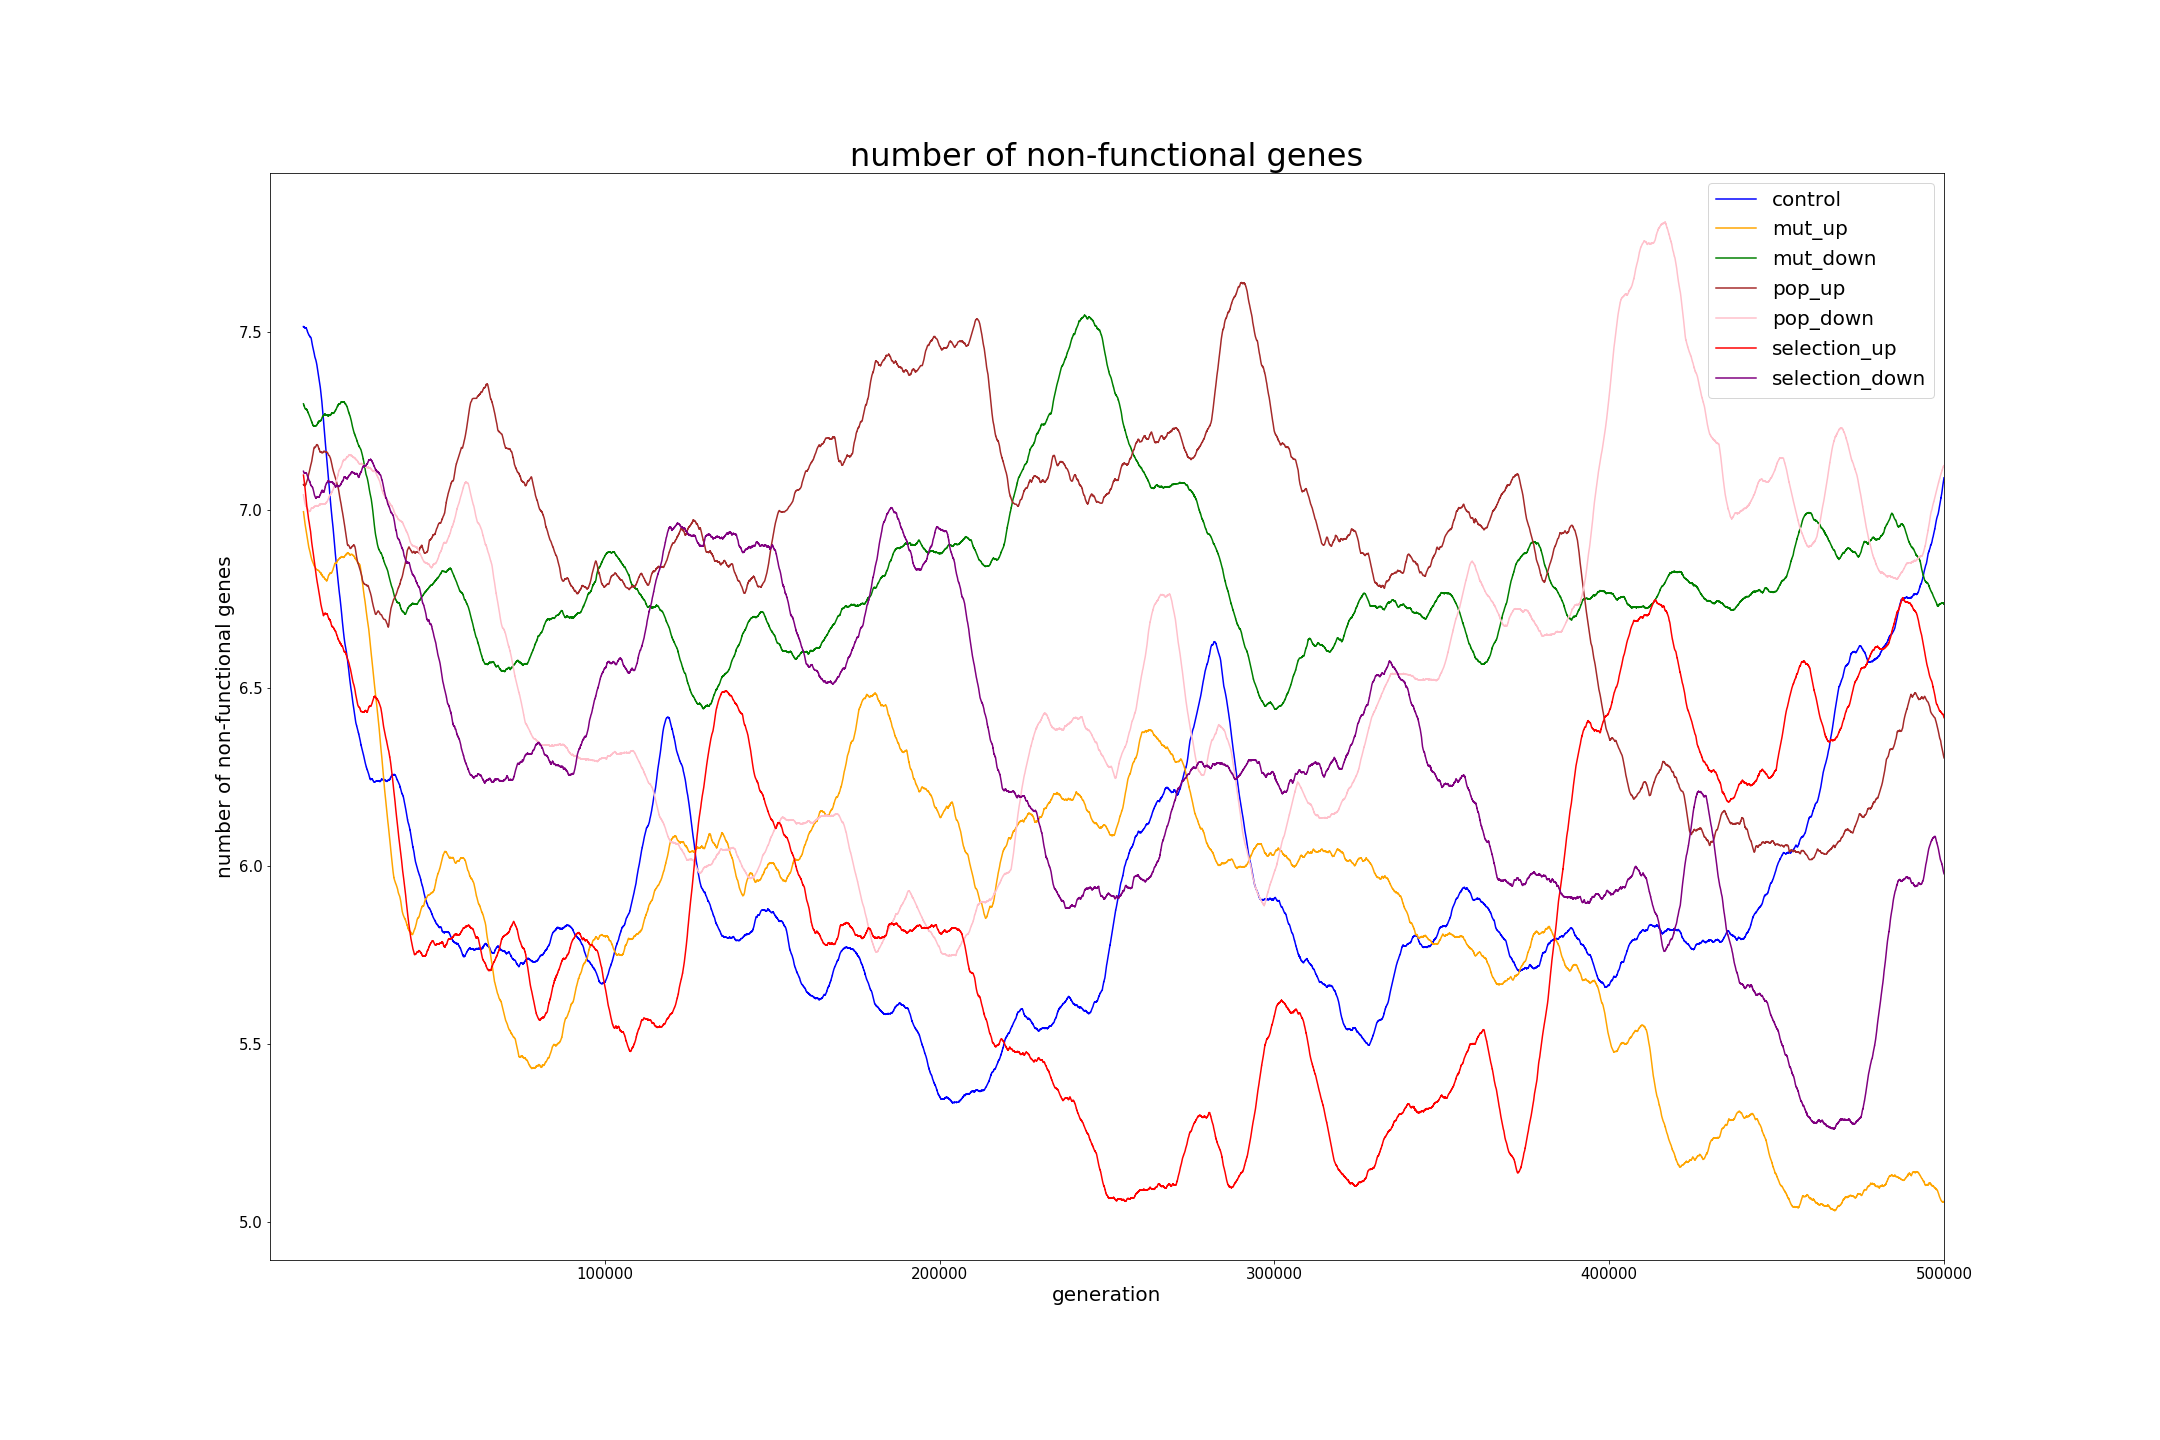
\includegraphics[width=\linewidth]{stat_genes_global_mean_num_non-functional_genes}
	\caption[Mean number of non-functional genes]{The mean number of non-functional genes across all seeds for each condition.}
	\label{fig:mean_num_non-functional_genes}
\end{figure}


\begin{table}[h]
	\centering
	\begin{tabular}{|c|c|c|}
		\hline
		\multicolumn{3}{c}{\Large \textbf{Number of Non-Functional Genes - Mean \& Std. Dev.}} \\
		\hline
		& \textbf{mean} & \textbf{standard deviation} \\
		\hline
		Control & 5.927067481209257 & 0.3857900832994517 \\
		\hline
		$\mu_+$ & 5.856448948104222	& 0.42847313257452385 \\
		\hline
		$\mu_-$ & 6.821347895210327 & 0.22159072539984662 \\
		\hline
		$k_+$ & 5.844289488031533 & 0.5069222102358901 \\
		\hline
		$k_-$ & 6.297804225025876 & 0.45415175059248414 \\
		\hline
		$N_+$ & & \\
		\hline
		$N_-$ & 6.555471025284081 & 0.4836308269184799 \\
		\hline
	\end{tabular}
	\caption[Number of Non-functional Genes - Mean \& St. Dev.]{The mean and standard deviation for the number of non-functional genes, all seeds, all conditions.}
	\label{table:non-functional_genes_mean_std_dev}
\end{table}

\subsubsection{Average Size of Functional Genes}\label{sec:average_size_functional_genes}
Figure~\ref{fig:mean_functional_gene_size} shows the average number of base pairs for each functional gene for the best individual, mapped out over the 500,000 generations. The population down condition continues to be the outlier in terms of genome structure, with the average size of the functional genes remaining noticeably lower than for any other condition. It is worth pointing out, however, that the difference between the smallest average and the largest average is only 1 base pair. 
\begin{figure}[H]
	\centering
	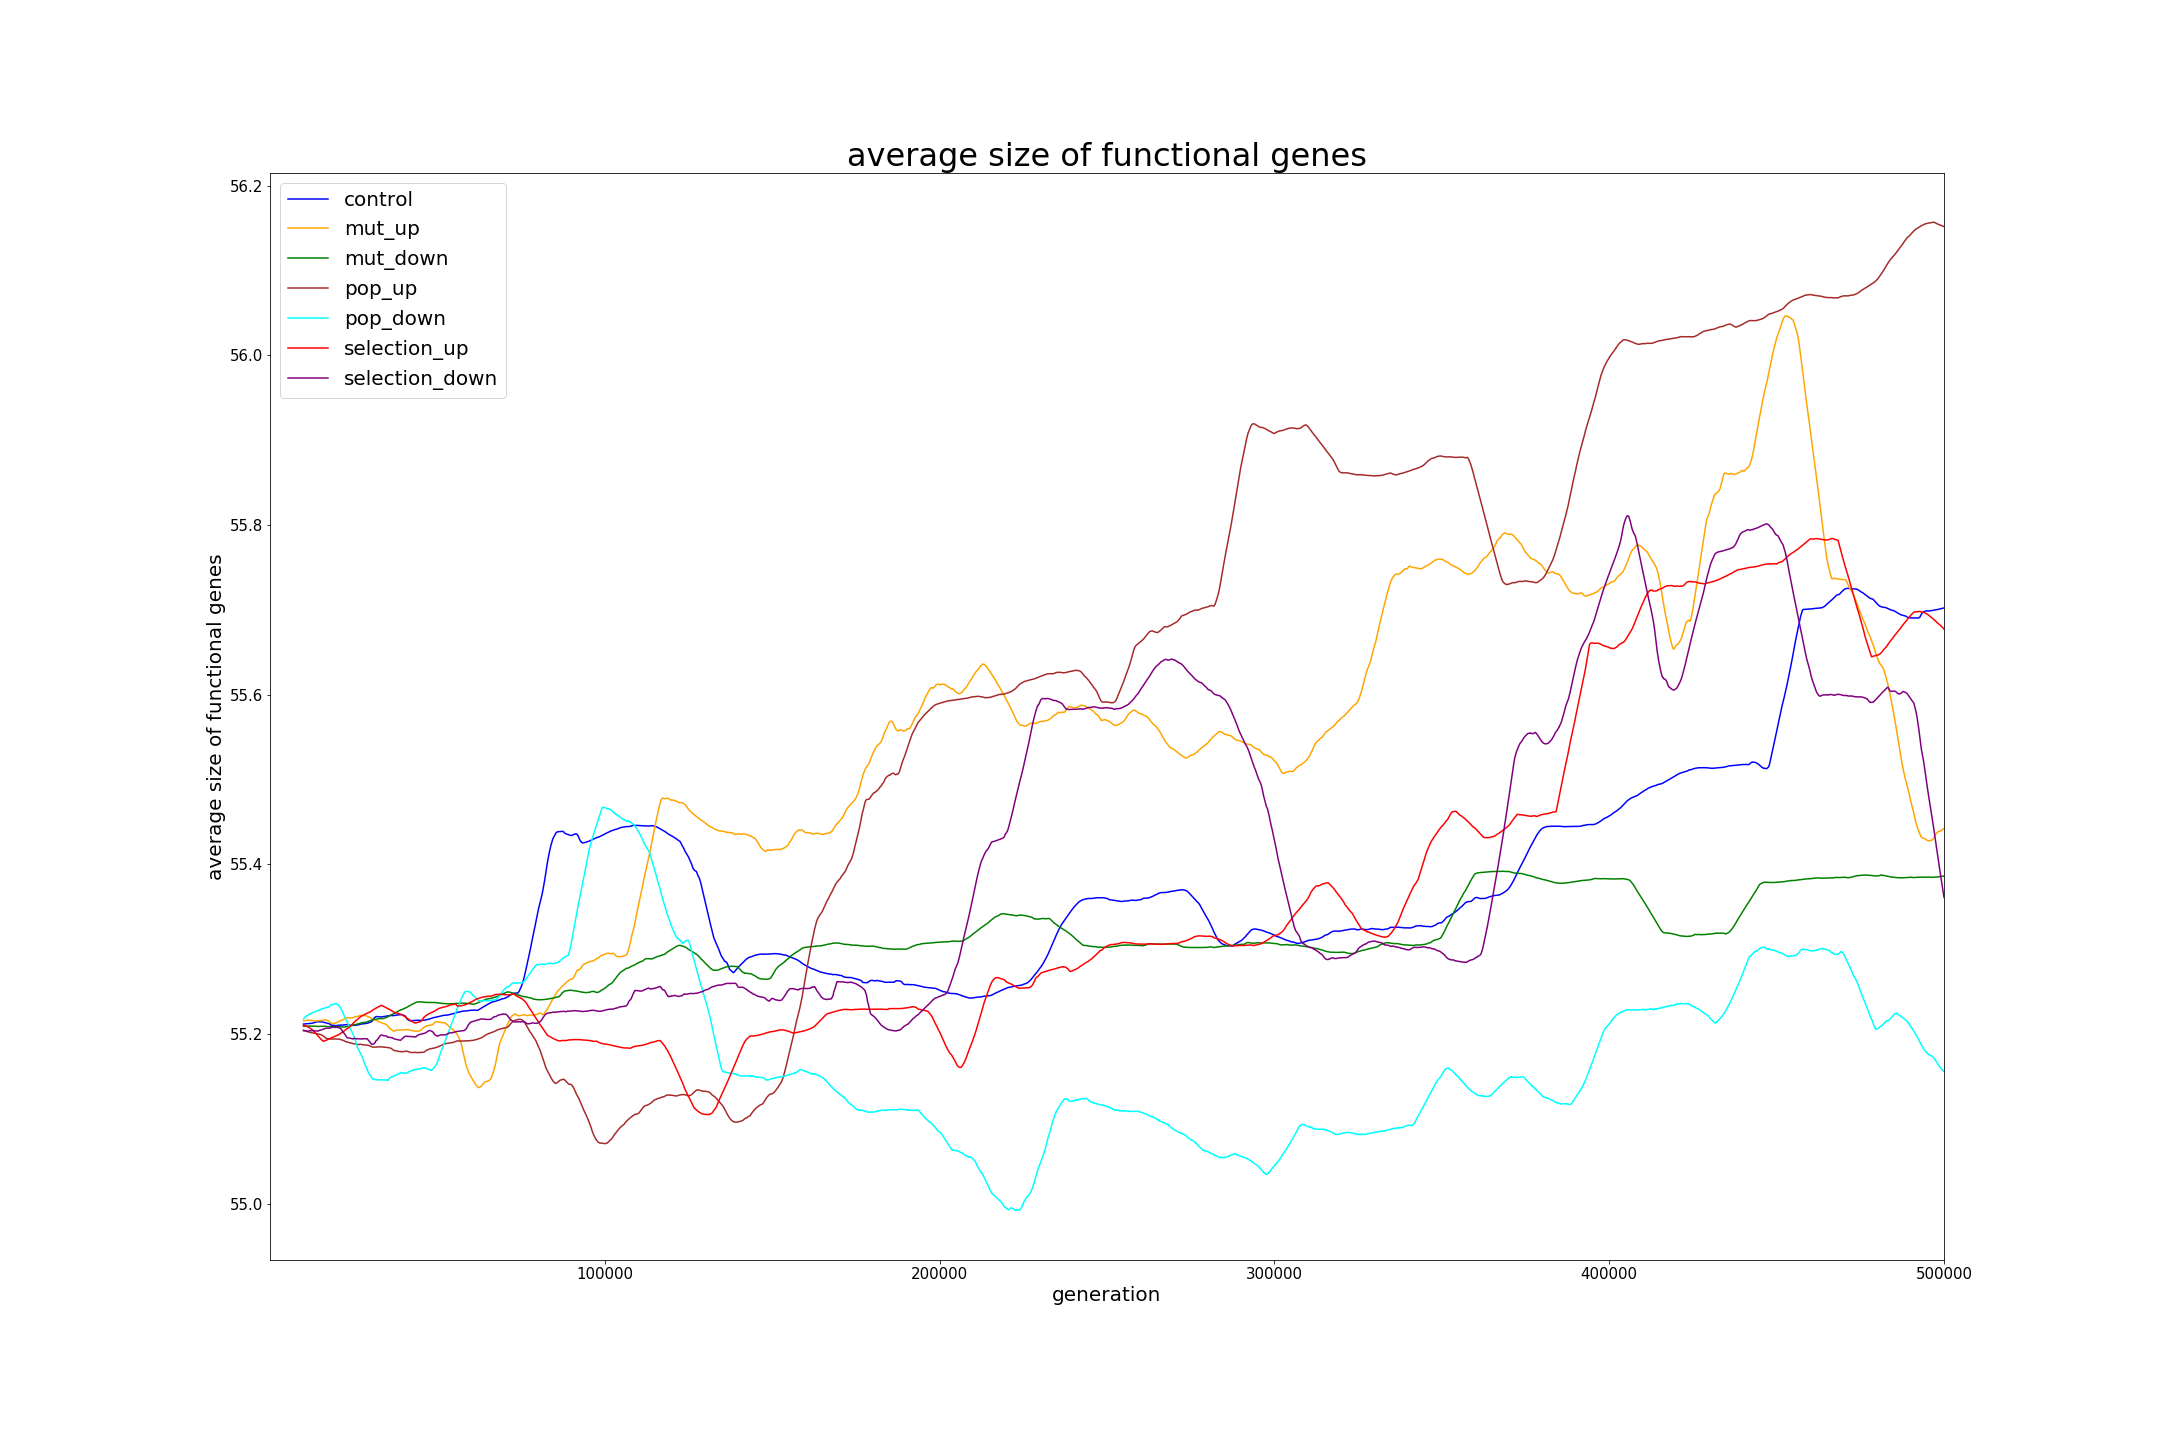
\includegraphics[width=\linewidth]{stat_genes_global_mean_avg_size_of_functional_genes}
	\caption[Average size of functional genes]{Plot showing the average size of functional genes over time for all seeds.}
	\label{fig:mean_functional_gene_size}
\end{figure}
Table~\ref{table:mean_functional_gene_size_and_std_dev} below gives the mean and standard deviation of the results, and Table~\ref{table:avg_size_of_functional_genes_rank_sum_and_p-value} gives the p-values for comparing the control condition to every other condition. 

\begin{table}[H]
	\centering
	\begin{tabular}{|c|c|c|}
		\hline
		\multicolumn{3}{c}{\Large \textbf{Average size of functional genes}} \\
		\hline
		& \textbf{mean} & \textbf{standard deviation} \\
		\hline
		Control & 55.375429751247275 & 0.13745740540215895 \\
		\hline
		$\mu_+$ & 55.5426245000319 & 0.20716437222446815\\ 
		\hline
		$\mu_-$ & 55.309915451000805 & 0.05059383390579744 \\
		\hline
		$k_+$ & 55.37046527382346 & 0.2024427915314053 \\
		\hline
		$k_-$ & 55.414464890880595 & 0.1954246818788886 \\
		\hline
		$N_-$ & 55.17428963311534	& 0.09886004440916518 \\
		\hline
	\end{tabular}
	\caption[Mean functional gene size and standard deviation]{Mean functional gene size and standard deviation, all seeds, all conditions.}
	\label{table:mean_functional_gene_size_and_std_dev}
\end{table}

\begin{table}[H]
	\begin{tabular}{|c|c|c|}
		\hline
		\multicolumn{3}{c}{\Large \textbf{Average size of functional genes - rank sum \& p-value}} \\
		\hline
		& \textbf{rank sum} & \textbf{p-value} \\
		\hline
		$\mu_+$ & 68252491056.0 & 0.00000000000000 \\
		\hline
		$\mu_-$ & 96067062201.5 & 0.00000000000000 \\
		\hline
		$N_-$ & 28963878467.0 & 0.00000000000000 \\
		\hline
		$k_+$ & 103481641646.0 & 0.00000000000000 \\
		\hline
		$k_-$ & 124890321462.0 & 0.223664707704009 \\
		\hline
	\end{tabular}
	\caption[Average size of functional genes - rank sum and p-value]{Average size of functional genes - rank sum and p-value for all conditions and all seeds.}
	\label{table:avg_size_of_functional_genes_rank_sum_and_p-value}
\end{table}
Since the $k_-$ condition's p-value was $\geq0.05$, we must conclude that these results are not significant. 

\subsection{Evolvability}
In Figure~\ref{fig:evolvability_mean} below, we see the results of the experiments on evolvability for the best individual's (at generation 500,000) lineage. 
\begin{figure}[H]
	\centering
	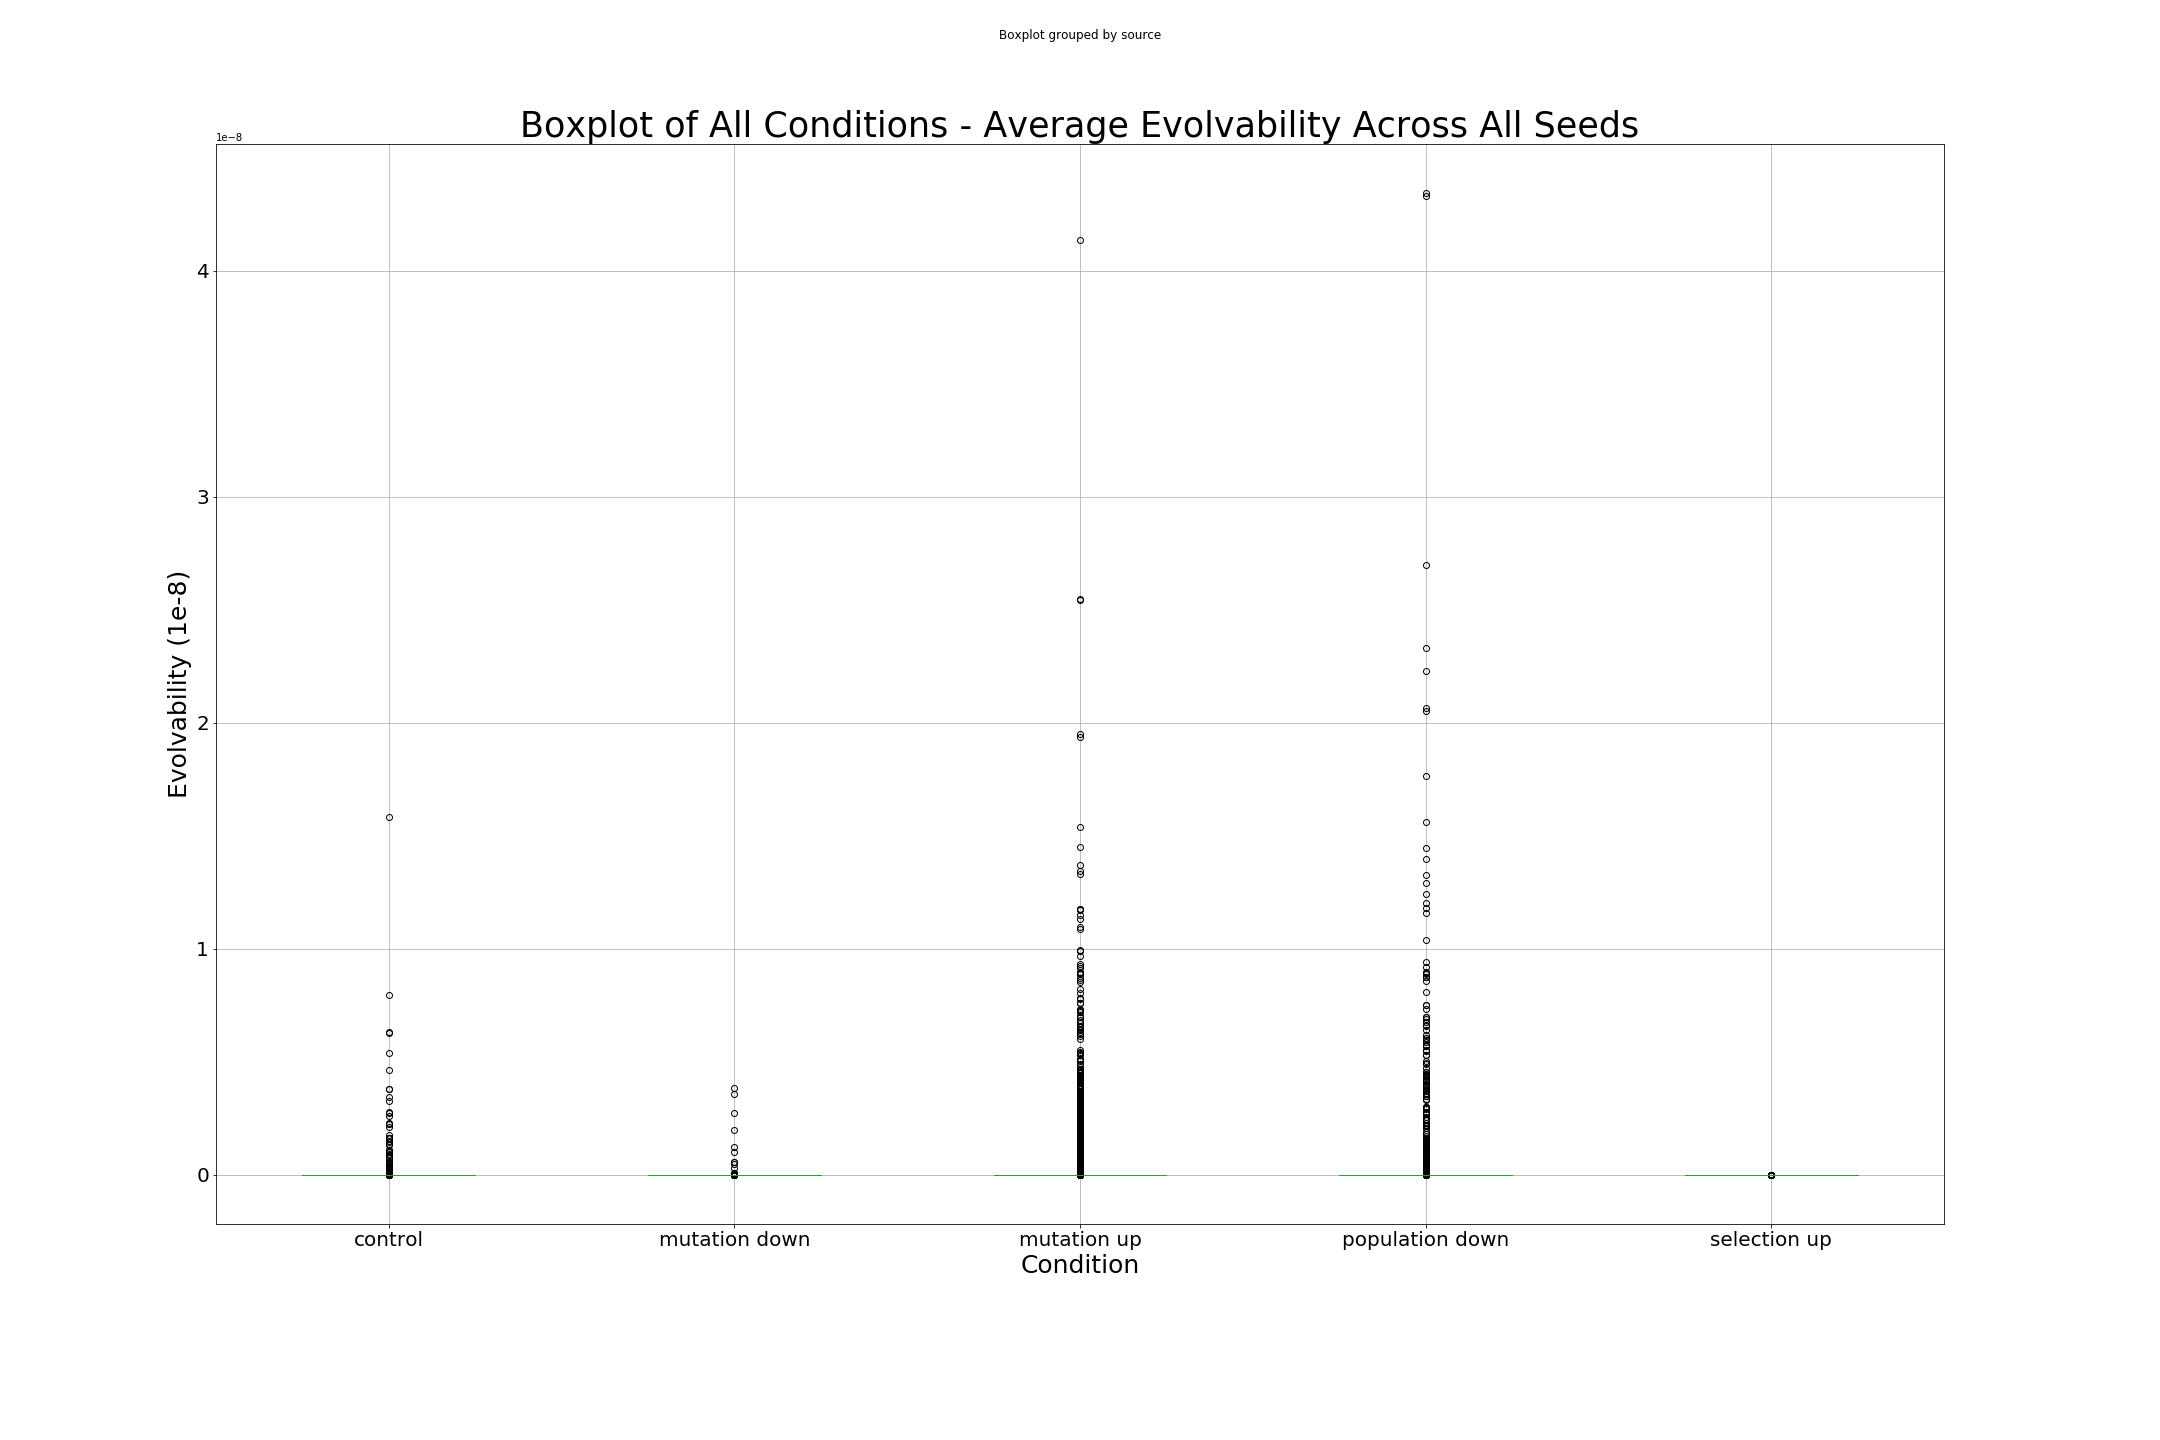
\includegraphics[width=\linewidth]{evolvability_boxplot_all_seeds_avg}
	\caption[Evolvability boxplot]{A box plot showing the mean evolvability spread of all seeds and all conditions. Higher numbers are more evolvable.}
	\label{fig:evolvability_mean}	
\end{figure}
The figure illustrates that, for each condition, overall the best individual still had quite low evolvability. For the selection up condition, however, the deviation from zero was even smaller, as illustrated in Table~\ref{table:mean_std_dev_evolvability} below, which provides the mean and standard deviation of the evolvability of the best individual in each condition. 

The evolvability rank sum and p-value information is given in Table~\ref{table:evolvability-rank_sum_and_p-values}.

\begin{table}[H]
	\begin{tabular}{|c|c|c|}
		\hline
		\multicolumn{3}{c}{\Large \textbf{Evolvability rank sum and p-value}} \\
		\hline
		& \textbf{rank sum} & \textbf{p-value} \\
		\hline
		$\mu_+$ & 36203620.0 & 0.000000000309416 \\
		\hline
		$\mu_-$ & 7025283.5 & 0.010212448990316 \\
		\hline
		$k_+$ & 13181851.5 & 0.000000000000074 \\
		\hline
		$k_-$ & 13779001.5 & 0.000000084666842 \\
		\hline
		$N_+$ & & \\
		\hline
		$N_-$ & 19403134.5 & 0.00000000000000 \\
		\hline
	\end{tabular}
	\caption[Evolvability - rank sum and p-value]{Rank sum and p-values for evolvability, all seeds, all conditions.}
	\label{table:evolvability-rank_sum_and_p-values}
\end{table}

\begin{table}[H]
	\centering
	\begin{tabular}{| c | c | c |}
		\hline
		\multicolumn{3}{c}{\Large Evolvability - Mean \& Std. Dev.} \\
		\hline
		& \textbf{mean} & \textbf{standard deviation}\\
		\hline
		\hline
		control & 2.035523813975702e-11 & 3.2787490312081233e-10\\
		\hline
		$\mu_+$ & 9.97655150597127e-11 & 8.41749150634588e-10 \\
		\hline
		$\mu_-$ & 6.064697990806935e-12 & 1.2471674281540128e-10 \\
		\hline
		$k_+$ & 1.9498939718794653e-15 & 6.394659146405824e-14 \\
		\hline
		$k_-$ & 4.3065723639721706e-10 & 5.20232907351617e-09 \\
		\hline
		%TODO Fill in population up
		$N_+$ &  & \\
		\hline
		$N_-$ & 8.837632116681012e-11 &  1.0799303682398726e-09 \\
		\hline	 		 
	\end{tabular}
	\caption[Evolvability mean and standard deviation]{Table illustrating the mean and standard deviation of the evolvability for each condition. $\mu$ is the mutation rate, $k$ is the selection rate, and $N$ is the population size.}
	\label{table:mean_std_dev_evolvability}
\end{table}

\subsection{Robustness}
Recall from Section~\ref{subsec:robustness_antirobustness} that robustness is measured by the fraction of neutral offspring of an individual. In the following figure, we see a bar plot showing the spread of neutral offspring for the best individual for the control condition as well as the six variations. 

%TODO update graphic with more conditions once experiments are completed
\begin{figure}[H]
	\centering
	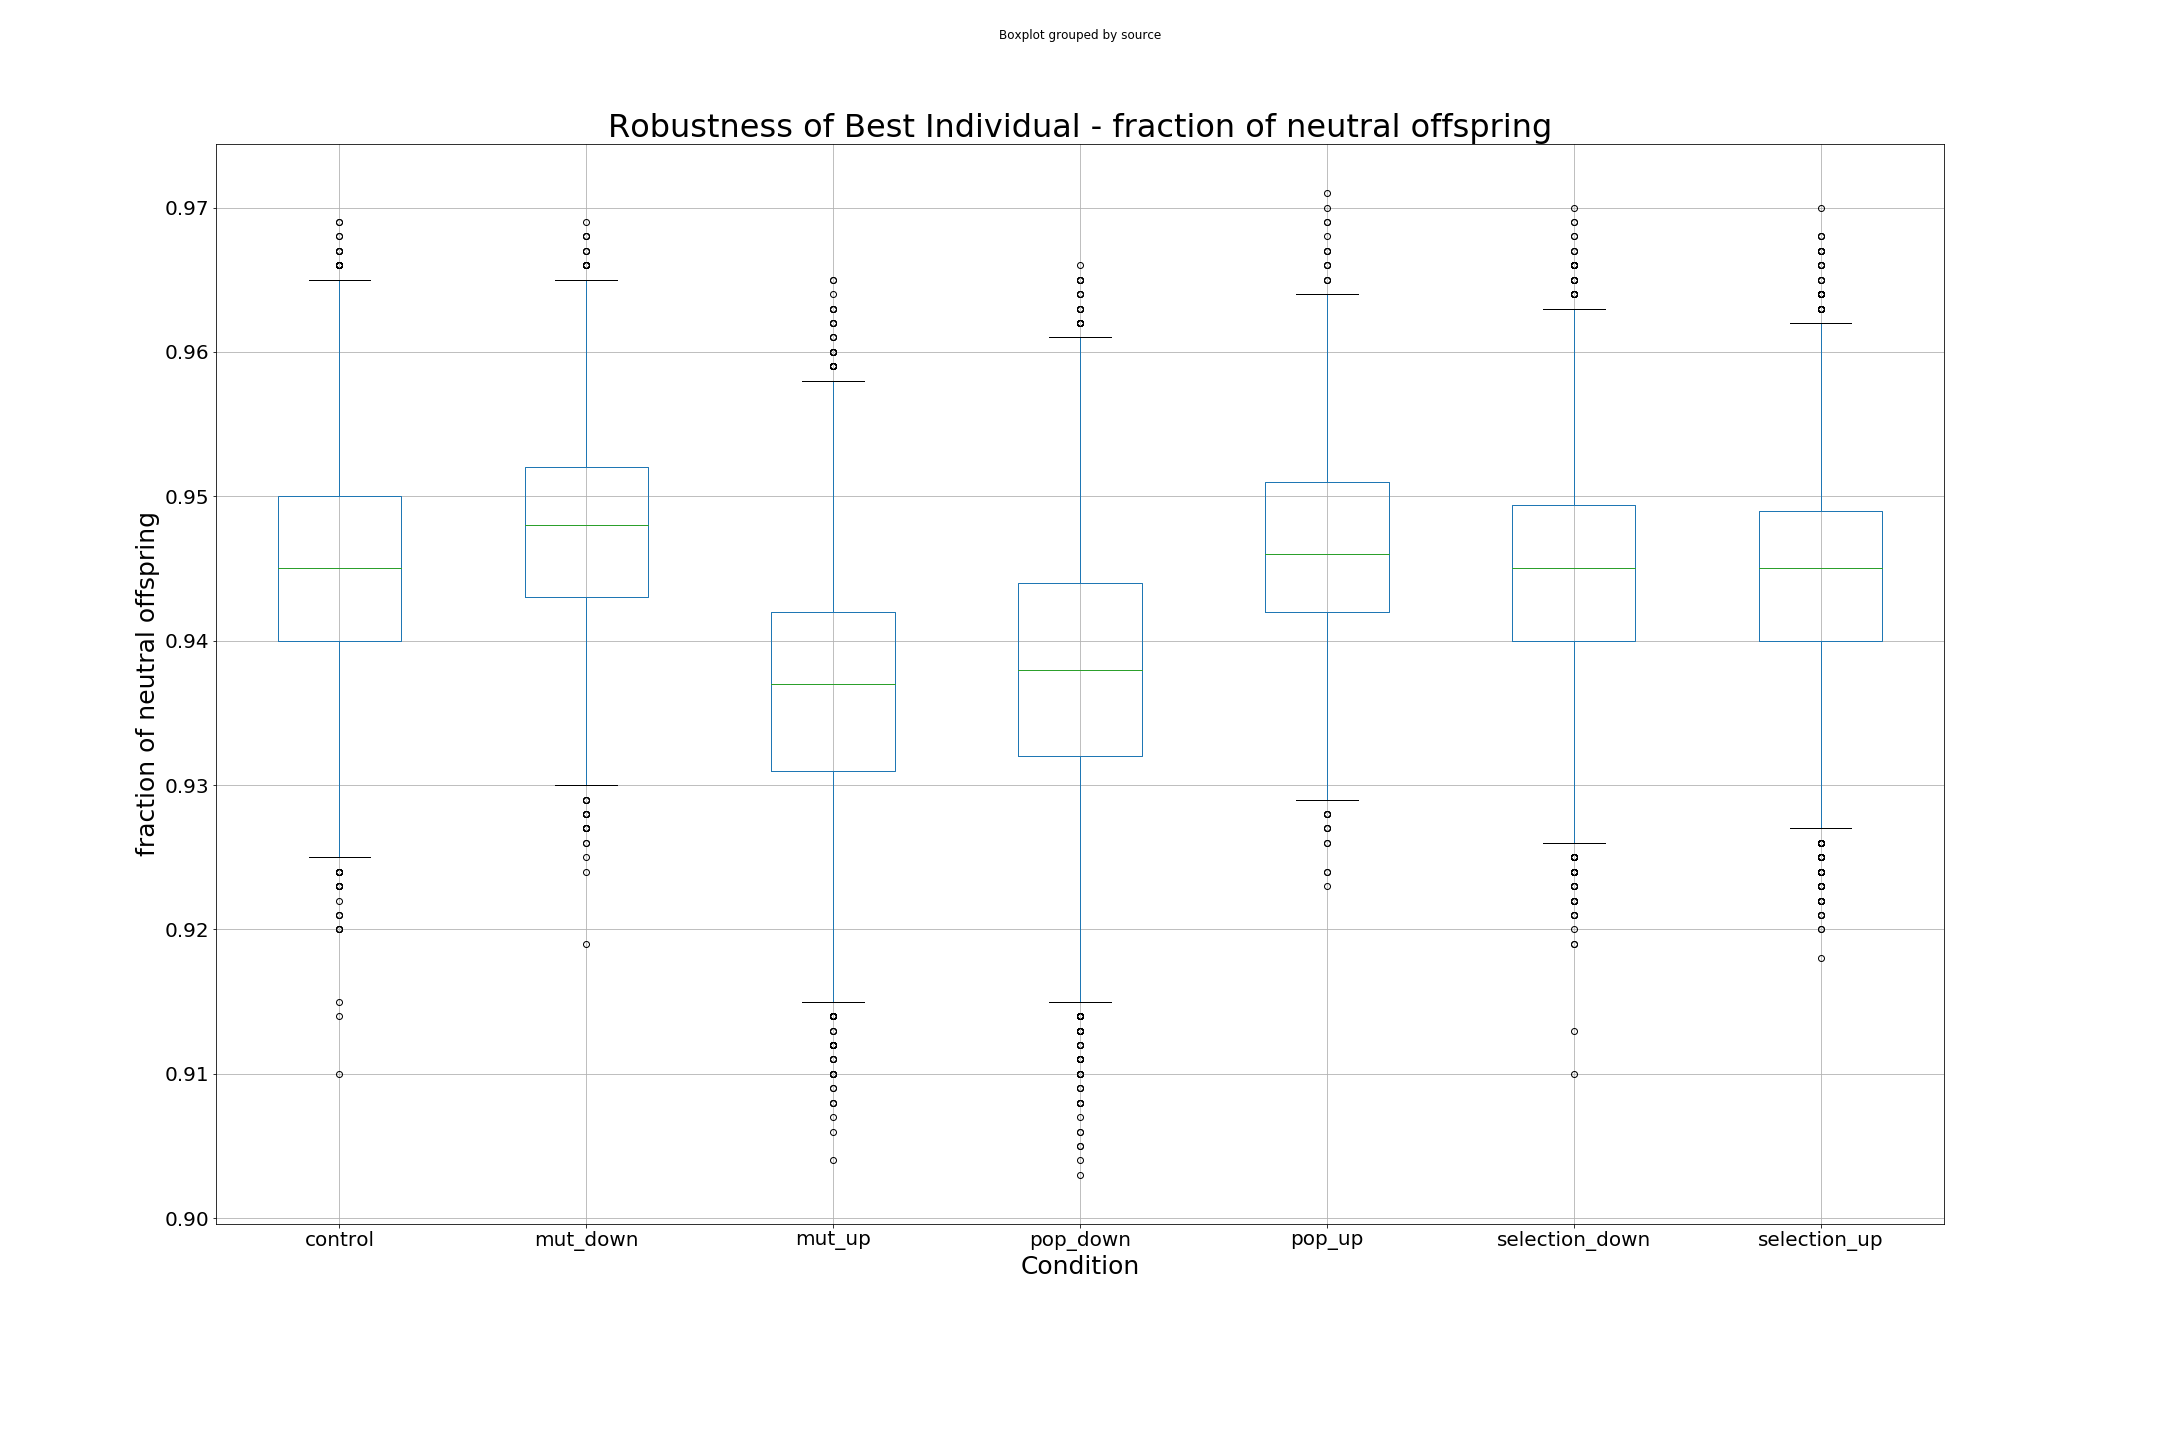
\includegraphics[width=\linewidth]{stat_robustness_best_mean_frac_neutral_offspring}
	\caption[Robustness bar graph]{Bar graph showing the spread of neutral offspring for the best individual at generation 500,000, all conditions.}
	\label{fig:mean_robustness_all_conditions}
\end{figure}
The mutation up condition clearly had the largest mean percentage of neutral mutants, at 0.5\%. The full statistics are given in the tables below:

\begin{table}
	\begin{tabular}{|c|c|c|}
		\hline
		\multicolumn{3}{c}{\Large \textbf{Robustness - Rank Sum \& p-values}} \\
		\hline
		& \textbf{rank sum} & \textbf{p-value} \\
		\hline
		$\mu_+$ & 16756710.5 & 0.000000000000000 \\
		\hline
		$\mu_-$ & 5741758.0 & 0.000000000000000 \\
		\hline
		$N_-$ & 12493750.0 & 0.000000000000000 \\
		\hline
		$k_+$ & 13580845.5 & 0.001358704915202 \\
		\hline
		$k_-$ & 13925884.0 & 0.001273247024315 \\
		\hline
	\end{tabular}
	\caption[Robustness rank sum \& p-values]{Mean robustness rank sum and p-values for all conditions and all seeds.}
	\label{table:rank_sum_p-values}
\end{table}
\begin{table}[H]
	\begin{tabular}{|c|c|c|}
		\hline
		\multicolumn{3}{c}{\Large \textbf{Robustness - means \& standard deviations}} \\
		\hline
		& \textbf{rank sum} & \textbf{p-value} \\
		\hline
		Control & 0.944925327538429	& 0.007334383035973237 \\
		\hline
		$\mu_+$ & 0.9366773604226319 & 0.007907308763606846 \\
		\hline
		$\mu_-$ &	0.94754266274366 & 0.0070662676155014035 \\
		\hline
		$k_+$ & 0.9444661080775791 & 0.007371509508882273 \\
		\hline
		$k_-$ & 0.9445156995960435	& 0.007423851661757711 \\
		\hline
		$N_-$ & 0.9374093190746451 & 0.008846010304259707 \\
		\hline
	\end{tabular}
	\caption[Robustness means and standard deviations]{Robustness means and standard deviations for all conditions and all seeds.}
	\label{table:robustness_means_and_std_dev}
\end{table}


\section{Discussion}\label{discussion}

Analogously to Table~\ref{table:experiment_predictions}, we summarize the results of our experiments in Table~\ref{table:experiment_results_summary} below. For each cell, {\color{green} green} indicates that our prediction was confirmed in our experiments and {\color{red}red} indicates that the prediction must be rejected. Our predictions for each condition are duplicated here for convenience, with a $+$ indicating a predicted increase and $-$ indicating a predicted decrease over the control condition. 

%TODO Is this table from Chapter 3 correct? Specifically, is mutation+/- right for fitness? 
\begin{table}[H]
	\centering
	\begin{tabular}{|c||c|c|c|c|c|c|}
		\hline
		\multicolumn{7}{|c|}{{\Large \textbf{Experiment Results Summary}}} \\
		\hline \hline
		\multirow{2}{*}{\textbf{Effect On:}} & \multicolumn{6}{c|}{\textbf{Condition}} \\
		\cline{2-7}
		& {\Large$\mu_+$} & {\Large$\mu_-$} & {\Large$k_+$} & {\Large$k_-$} & {\Large$N_+$} & {\Large$N_-$} \\
		\hline 
		Genome Size & \cellcolor{green} $-^{\cite{bradwell2013correlation, marais2008mutation}}$ & \cellcolor{red} $\text{+}^{\cite{bradwell2013correlation, drake1991constant}}$ & \cellcolor{green} $+^{\cite{Batut.2013}}$ & \cellcolor{green} $-^{\cite{Batut.2013}}$ & $-^{\cite{Batut.2014}}$ & \cellcolor{green} $+^{\cite{Batut.2014}}$ \\
		\hline
		Fitness & \cellcolor{green} $+^{\cite{bataillon2000estimation, vahdati2017effect}}$ & \cellcolor{green} $-^{\cite{vahdati2017effect}}$ & \cellcolor{red} $+^{\cite{Batut.2014}}$ & \cellcolor{red} $-^{\cite{Batut.2014}}$ & $+^{\cite{cutter2019primer, vahdati2017effect}} $ & \cellcolor{green} $-^{\cite{cutter2019primer, vahdati2017effect}} $\\
		\hline
		Amount of non-coding DNA & \cellcolor{green} $-^{\cite{Knibbe2007}}$ & \cellcolor{red} $+^{\cite{Knibbe2007}}$ & \cellcolor{green} $+^{\cite{Batut.2013, Knibbe2007}}$ & \cellcolor{green} $-^{\cite{Batut.2013, Knibbe2007}}$ & $-^{\cite{Batut.2013}}$ & \cellcolor{green} $+^{\cite{Batut.2013}}$ \\
		\hline
		Number of genes & \cellcolor{red} $-^{\cite{Knibbe2007}}$ & \cellcolor{green} $+^{\cite{Knibbe2007}}$ &\cellcolor{green} $+^{\cite{Knibbe2007}}$ & \cellcolor{green} $-^{\cite{Knibbe2007}}$ & $-^{\cite{Batut.2014}}$ & \cellcolor{green} $+^{\cite{Batut.2014}}$ \\
		\hline
		Average size of genes & \cellcolor{red} $-^{\cite{Liard.2018}}$ & \cellcolor{green} $+^{\cite{Liard.2018}}$ & \cellcolor{green} $-^{\cite{Batut.2013}}$ & \cellcolor{red}$+^{\cite{Batut.2013}}$ & $-^{\cite{Batut.2014}}$ & \cellcolor{red} $+^{\cite{Batut.2014}}$ \\
		\hline
		Robustness & \cellcolor{green} $-^{\cite{Knibbe2007}}$ &\cellcolor{green} $+^{\cite{Knibbe2007}}$ & \cellcolor{green} $-^{\cite{Batut.2013, Knibbe2007}}$ & \cellcolor{green}$+^{\cite{Batut.2013, Knibbe2007}}$ & $-^{\cite{elena2007effects}}$ & \cellcolor{red} $+^{\cite{elena2007effects}}$ \\
		\hline
		Evolvability &\cellcolor{green} $+^{\cite{Knibbe2007}}$ &\cellcolor{green} $-^{\cite{Knibbe2007}}$ & \cellcolor{red}  $+^{\cite{Batut.2013}}$ & \cellcolor{red} $-^{\cite{Batut.2013}}$ & $-^{\cite{wein2019effect}}$ & \cellcolor{green} $+^{\cite{wein2019effect}}$ \\
		\hline		
	\end{tabular}
	\caption[Experiment result summary]{A summary of whether our experiment results confirmed or denied the hypotheses of Table~\ref{table:experiment_predictions}.  were confirmed ({\color{green}green}) or rejected ({\color{red}red}), along with the predicted results of whether the given result would increase (+) or decrease (-) over the control condition.}
	\label{table:experiment_results_summary}
\end{table}

According to our predictions based on a survey of the literature (summarized in Table~\ref{table:experiment_predictions}), the $\mu_+$, $k_-$, and $N_+$ conditions should have lead to a reduced genome. As shown in Figure~\ref{fig:genome_size} however, none of these predictions held up, and in fact the genome size increased in all conditions, including those that were predicted to be reduced. One possible explanation is that, because the wild types had already been evolving for 10 million generations, and we did not vary the environment further for our experiments, perhaps they had reached a sort of stasis for which another half-million generations were not sufficient to fully demonstrate the effects of any changes. This may not explain everything, however, as some conditions (e.g. $\mu_+$, $N_-$) did see a rather rapid change in fitness, genome structure, etc. even in the (comparatively) short time. 

Also of interest is that, along with the genome size, overall the fitness of the organisms did not change much with only one exception ($k_+$). It has been postulated that perhaps gene loss may be selected for in order to increase the overall fitness of an organism by removing the added cost of the superfluous genes~\cite{koskiniemi2012}. Our results do not fully agree with this hypothesis, as our results show that, in addition to the general accumulation of non-coding DNA across all conditions (Figure~\ref{fig:mean_non-coding_DNA}), which would theoretically have a higher fitness cost, the number of genes actually \textit{increased} slightly for each condition, except for $k_-$. Likewise, fitness overall went \textit{up} as the number of genes increased (except for $N_-$). Lastly, decreasing the selection pressure resulted in the highest overall mean fitness by a wide margin (Table~\ref{table:fitness_means_std_dev}). In Aevol, non-coding DNA is not really associated with a fitness cost, so this explanation may likely also not fully apply. 

Regarding the $N_-$ condition, comparing this with the results of Batut et al. and their work with \textit{Buchnera aphidicola} (see Section~\ref{related_work}), it may be possible that gene loss is occurring because of the smaller effective population size clicking down Muller's Ratchet. This does not seem to be what is happening in our experiments either, however. Though mean fitness of the $N_-$ condition did greatly decline (see Figure~\ref{fig:mean_fitness_plot}), the $N_-$ condition also saw the largest accumulation of non-coding DNA (see Figure~\ref{fig:mean_non-coding_DNA}) and the second-highest level of evolvability (see Table~\ref{table:mean_std_dev_evolvability}), which should theoretically have lead to an easier time of overcoming the ratchet. On the other hand, the number of functional genes stayed more or less the same as all of the other conditions, and the accumulated number of non-functional genes (pseudogenes) of the $N_-$ condition was the largest (see Figure~\ref{fig:mean_num_non-functional_genes}). These two factors together suggest that there almost certainly was some loss of fitness through pseudogenization; perhaps with more time, the pseudogenes would also have been lost.

Recall the work of Liard et al.\cite{Liard.2018} as discussed in Section~\ref{related_work}, in which the proposed ``complexity ratchet'' was overcome by increasing the mutation rate. Their work was quite successful in overcoming this ratchet, but in our experiments, both the number of genes and the average size of the genes increased. One possible explanation for this is that, in their work, their increased mutation rate $\mu_+$ was set to $1e^{-3}$.  By contrast, even our elevated mutation rate, $\mu_+$, was just $4e^{-7}$, which is $\frac{1}{4}*e^4 \approx 13.65$ times lower than their highest mutation rate. Perhaps an even higher mutation rate would be sufficient to overcome the power of selection and reduce the genome further. 

%TODO Perform another experiment with a much higher mutation rate: 1e-3 for 100k generations?

